\documentclass[10pt]{article}
\pdfoutput=1 

\addtolength{\oddsidemargin}{-.875in}
\addtolength{\evensidemargin}{-.875in}
\addtolength{\textwidth}{1.75in}

\addtolength{\topmargin}{-.875in}
\addtolength{\textheight}{1.75in}

\openup 1em

%macro for commenting
\usepackage{color}
\newcommand{\leo}[1]{{\color{blue}{\it leo: #1}}}

\newcommand{\Xbeta}{ X_i \beta}
\newcommand{\xbeta}{ x_i \beta}
\newcommand{\xbetaij}{ x_{ij}^T \beta}
\newcommand{\sgamma}{s_{ij}^T\gamma_i}

\usepackage[round]{natbib}

\usepackage{rotating}
\usepackage{graphicx}
\usepackage{subcaption}

\usepackage{float}


\usepackage{amsthm,amsmath} 
\usepackage{amssymb}
\usepackage{subcaption}

\newtheorem{theorem}{Theorem}
\newtheorem{lemma}{Lemma}
\newtheorem{corollary}{Corollary}
\newtheorem{remark}{Remark}


\usepackage{algorithm}
\usepackage{algpseudocode}

\usepackage{mhequ}
\newcommand{\be}{\begin{equs}}
\newcommand{\ee}{\end{equs}}
\newcommand{\bb}[1]{\mathbb{#1}}
\newcommand{\mc}[1]{\mathcal{#1}}
\DeclareMathOperator{\Binom}{Binomial}
\DeclareMathOperator{\No}{No}
\DeclareMathOperator{\PG}{PG}
\DeclareMathOperator{\Bern}{Bernoulli}
\DeclareMathOperator{\U}{Uniform}
\DeclareMathOperator{\NB}{NB}
\DeclareMathOperator{\cov}{cov}
\DeclareMathOperator{\var}{var}
\DeclareMathOperator{\diag}{diag}
\DeclareMathOperator{\bigO}{\mc O}
\newcommand{\James}[1]{\textcolor{blue}{#1}}


\thispagestyle{empty}
\baselineskip=28pt

\title
{{Calibrated Data Augmentation for Scalable \\ Markov Chain Monte Carlo}}


\author{
     Leo L. Duan,
     James E. Johndrow,
     David B. Dunson
    % \textsuperscript{*}\footnotemark[2]\and
}

 
\begin{document}
    
\maketitle

% generally I don't use abbreviations in an abstract; some journals don't allow it
{\bf Abstract:} Data augmentation is a common technique for building tuning-free Markov chain Monte Carlo algorithms. Although these algorithms are very popular, 
autocorrelations are often high in large samples, leading to poor computational efficiency.  This phenomenon has been attributed to a discrepancy between Gibbs step sizes and the rate of posterior concentration in large samples.  In this article, we propose a family of calibrated data augmentation algorithms, which adjust for this discrepancy by inflating Gibbs step sizes with an auxiliary parameter. The bias introduced by the scale parameter can be eliminated through a Metropolis-Hastings step. The approach is applicable to a broad variety of existing data augmentation algorithms, and we focus on three popular models: probit, logistic and Poisson log-linear.  Theoretical support is provided and dramatic gains are shown in applications.
\vskip 12pt

%\baselineskip=12pt
%\par\vfill\noindent
{\noindent  KEY WORDS:  Bayesian probit; Bayesian logit; Approximate Markov chain Monte Carlo; Big $n$; Data Augmentation; Maximal Correlation; Polya-Gamma.}
%\par\medskip\noindent
%\clearpage\pagebreak\newpage
\pagenumbering{arabic}

\section{Introduction}

With the deluge of data in many modern application areas, there is pressing need for scalable computational algorithms for inference from such data, including uncertainty quantification (UQ).  Somewhat surprisingly, even as the volume of data increases, uncertainty often remains sizable.  Examples in which this phenomenon occurs include financial fraud detection \citep{ngai2011application}, disease mapping \citep{wakefield2007disease} and online click-through tracking \citep{wang2010click}.  Bayesian approaches provide a useful paradigm for quantifying uncertainty in inferences and predictions in these and other settings.

The standard approach to Bayesian posterior computation is Markov chain Monte Carlo (MCMC) and related sampling algorithms. Non-sampling alternatives, such as variational Bayes, tend lack general accuracy guarantees. However, it is well known that conventional MCMC algorithms often scale poorly in problem size and complexity. Due to its sequential nature, the computational cost of MCMC is the product of two factors: the evaluation cost at each sampling iteration and the total number of iterations needed to obtain an acceptably low Monte Carlo error. The latter is related to the properties of the Markov transition kernel; we will refer to this informally as the \emph{mixing properties} of the Markov chain. 

In recent years, a substantial literature has developed focusing on decreasing computational cost per iteration (\cite{minsker2014robust,srivastava2015wasp,conrad2015accelerating} among others), mainly through accelerating or parallelizing the sampling procedures at each iteration. Moreover, myriad strategies for improving mixing have been described in the literature. For Metropolis-Hastings (M-H) algorithms, improving mixing is usually a matter of contructing a better proposal distribution. An important difference between M-H and Gibbs is that one has direct control over step sizes in M-H through choice of the proposal, while Gibbs step sizes are generally not tunable; on the other hand, finding a good proposal for multi-dimensional parameters in M-H is significantly more challenging compared to Gibbs sampling. Thus, improving mixing for Gibbs has historically focused on decreasing autocorrelation by changing the update rule itself, for example by parameter expansion (PX), marginalization, or slice sampling.\footnote{Although strictly speaking, slice sampling is just an alternative approach to sampling from a full conditional distribution, in practice, it is often an alternative to data augmentation, so that using a slice sampling strategy results in the removal of a data augmentation step from an alternative Gibbs sampler.} 

The treatment of the behavior of MCMC for large $n$ and/or $p$ in the theory literature is arguably somewhat limited. Historically, many authors have focused on studying the mixing properties of MCMC by showing a general ergodicity condition, such as the geometric ergodicity condition of (cite Meyn and Tweedie, Roberts and Rosenthal). This generally yields bounds on the convergence rate and spectral gap of the Markov chain under consideration, but \cite{rajaratnam2015mcmc} observe that in many cases, these bounds converge to zero exponentially fast in $p$ or $n$, so that no meaningful guarantee of performance for large problem sizes is provided by most existing bounds. In the probability literature, a series of papers have developed an analogue of Harris' theorem and ergodic theory for infinite-dimensional state spaces (cite Hairer, Mattingly and friends papers). Recent work verifies the existence of MCMC algorithms for computation in differential equation models with dimension-independent spectral gap (Hairer, Stuart, Vollmer). In this example, the algorithm under consideration is a M-H algorithm, and it is clear that the proposal must be tuned very carefully to achieve dimension independence. Other work has studied the properties of the limiting differential equation that describes infinite-dimensional dynamics of MCMC.

A recent paper (\cite{johndrow2016inefficiency}) studies the popular data augmentation algorithms for posterior computation in probit, \citep{albert1993bayesian} and logistic models \citep{polson2013bayesian}, showing that the algorithm fails to mix in large sample sizes when the data are imbalanced. An important insight is that the performance can be largely explained by a discrepancy between the rate at which Gibbs step sizes and the width of the high-probability region of the posterior converge to zero as the sample size increases. Thus, since Gibbs step sizes are generally not tunable, slow mixing is likely to occur as the sample size grows unless the order of the step size happens to match the order of the posterior width. This implies that if a way to directly control the step sizes of the Gibbs sampler could be devised, it would be possible to make the mixing properties of the sampler insensitive to sample size by scaling the step sizes appropriately. This is similar to the conclusion of (HSV), except in this case, we have growing $n$ instead of growing $p$.

In this article, we propose a method for tuning Gibbs step sizes by introducing auxiliary parameters that change the variance of full conditional distributions for one or more parameters. Although we focus on data augmentation algorithms for logit, probit, and poisson log-linear models, in principle the strategy can be applied more generally to align Gibbs step sizes with the size of the space being explored. As these ``calibrated'' data augmentation alters the invariant measure, one can use the Gibbs step as an efficient M-H proposal, thereby recovering the correct invariant, or view the resulting algorithm as a perturbation of the original Markov chain. We use bias correction through a second set of working parameters.

\section{Calibrated Data Augmentation}
The method is developed primarily in the context of Data augmentation Gibbs samples, which are based on the integral $ \pi(\theta|y)=\int\pi(\theta|z,y)\pi(z|y) dz$ and take the general form
\be \label{eq:da}
z \mid \theta, y &\sim p(z;\theta,y) \\
\theta \mid z,y &\sim f(\mu(z),\Sigma(z)),
\ee
where $f$ belongs to the location-scale family such as Gaussian. This allows conditional updates for the frequently high-dimensional parameter $\theta$. As such, data augmentation is an important computational strategy when the difficulty of tuning Metropolis-Hastings algorithms is prohibitive due to dimension or complexity of the target distribution. An important class of data augmentation algorithms are those for generalized linear models (GLMs) with $\bb E[y_i \mid x_i, \theta] = g^{-1}(x_i \theta)$ and conditionally Gaussian prior on $\theta$. We focus in particular on poisson log-linear, binomial logistic, and binomial probit as motivating examples.

The calibration of step sizes is best illustrated by an example. Consider the binomial probit, with sampling model
\be
y_i \sim \Bern(p_i), \quad p_i = \Phi(x_i \beta),
\ee
and improper prior $\pi(\beta)=1$. The basic data augmentation algorithm (tanner and wong, albert and chib, etc) has the update rule
\be
z_i \mid \beta, x_i, y_i &\sim \left\{ \begin{array}{cc} \No_{[0,\infty)}(x_i \beta,1) & \text{ if } y_i = 1 \\ \No_{(-\infty,0]}(x_i \beta,1) & \text{ if } y_i = 0 \end{array} \right. \\
\beta \mid z, x, y &\sim \No((X'X)^{-1} X'z, (X'X)^{-1}),
\ee
where $\No_{[a,b]}(\mu,\sigma^2)$ is the normal distribution with mean $\mu$ and variance $\sigma^2$ truncated to the interval $[a,b]$. To make the Gibbs step sizes tunable, we introduce an auxiliary parameter $r_i$ as the conditional variance of $z_i$. 
% we can't reset b_i = (\sqrt{r_i}-1) x_i\beta every time, since it won't lead to convergence of Markov chain. instead, we have to fix b_i at some point, leading to different target distribution that needs to be corrected.
To reduce the bias caused by $r_i$, we adjust the mean by another auxiliary parameter $b_i$, giving

\be
\int_{-\infty}^{0} \frac{1}{\sqrt{2 \pi r_i} } \exp\left(-\frac{(z_i-\xbeta-b_i)^2}{2 r_i^2} \right) dz_i = \Phi( \frac{\xbeta+b_i}{\sqrt{r_i}}),
\label{eq:prop-marginal-probit}
\ee
yielding the update rule 
\be \label{eq:cda-probit}
z_i \mid \beta, x_i, y_i &\sim \left\{ \begin{array}{cc} \No_{[0,\infty)}(x_i \beta+b_i,r_i) & \text{ if } y_i = 1 \\ \No_{(-\infty,0]}(x_i \beta+b_i,r_i) & \text{ if } y_i = 0 \end{array} \right. \\
\beta^* \mid z, X &\sim \No((X'R^{-1}X)^{-1} X'R^{-1}(z-b), (X'R^{-1}X)^{-1}),
\ee
where $R = \diag(r_1,\ldots,r_n)$, $b = (b_1,\ldots,b_n)'$. Note that the parameter expansion algorithms of \cite{liu1999parameter} and \cite{meng1999seeking} rescale $\beta$ by $1/\sqrt{r}$, which does not change in the conditional variance for $\beta$. Our formulation allows a direct control of the step sizes through the value of $r$.

The update in \eqref{eq:cda-probit} alters the invariant measure; thus, we use it as a M-H proposal. Letting $Q(\beta^*;\beta)$ be the proposal defined by \eqref{eq:cda-probit}, the proposal is accepted with probability
%Generate one uniform random variable $u\sim \U(0,1)$ and accept the new $\beta^*$ if
\be
1 \wedge \frac{Q(\beta; \beta^*) \pi(\beta^*) \prod_i L(\xbeta^*;y_i)}{Q(\beta^*; \beta)\pi(\beta) \prod_i L(\xbeta;y_i) } = 1 \wedge  \frac{  \prod_i L_r(\xbeta;y_i) L(\xbeta^*;y_i)}{\prod_i  L_r(\xbeta^*;y_i)L(\xbeta;y_i) },
\label{eq:mh-criterion}
\ee
where $L(\theta;y_i)=\Phi(\theta)^{y_i} (1-\Phi(\theta))^{(1-y_i)}$ and  $L_r(\theta;y_i)=\Phi( \frac{\theta+b_i}{\sqrt{r_i}} )^{y_i} (1-\Phi(\frac{\theta+b_i}{\sqrt{r_i}}))^{(1-y_i)}$. The second equality holds since $Q(\beta; \beta^*) Q(\beta^*) = Q(\beta; \beta^*)Q(\beta)$ and $ Q(\beta) = C\pi(\beta) \prod_i L_r(\xbeta;y_i)$ as the posterior density under the altered $L_r$ with $C$ as the constant free from $\beta$. It is worth noting that setting $r_i=1$ and $b_i=0$ leads to acceptance rate of $1$, which corresponds to the original Gibbs sampling step.


When the proposal is accepted $\beta_t = \beta^*$, the covariance:
\be
\cov(\beta_t \mid \beta_{t-1}, r,X,z) = (X'R^{-1}X)^{-1} + (X'R^{-1}X)^{-1} X'R^{-1}\cov(z-b | R) R^{-1}X(X'R^{-1}X)^{-1} 
\ee
so that the step size:
\be
 \var(\beta_t \mid \beta_{t-1}, r,X,z)   \ge  \diag((X'R^{-1}X)^{-1}), \label{eq:varlb-probit}
\ee
is lower bounded by linear combination of the $r_i$. In an intercept-only model, the variance is bounded by $\left(\sum_i r_i^{-1}\right)^{-1}$ via \eqref{eq:varlb-probit}, $1/n$ times the harmonic mean of the $r_i$. \cite{johndrow2016inefficiency} show that when $\sum_i y_i = 1$ and $r_i = 1$, $\var(\beta_t \mid \beta_{t-1})$ is approximately $n^{-1} \log n$, while the width of the high probability region of the posterior is order $(\log n)^{-1}$, leading to slow mixing. Thus, to achieve step sizes consistent with the width of the space, we need
\be
\left(\sum_i r_i^{-1}\right)^{-1} &\approx (\log n)^{-1} \\
\intertext{ so if $r_i = r$ for all $i$ }
\frac{n}{r} \approx \log n \Rightarrow r \approx \frac{n}{\log n}. 
\ee

To illustrate the effect of this calibration, consider an intercept only probit model, with $\sum_i y_i =1$ and $n=10^4$. We set $r_i=r$ for all $i$. To increase the acceptance rate of the M-H step, we use a rough estimate of $b_i = -3.7 (\sqrt r -1)$ to have the effective probability near $\Phi(-3.7)= 10^{-4}$ in the proposal distribution (later we will show the adaptation for $b_i$ without using prior knowledge). Setting $r=1$ in the proposal corresponds to the original \cite{albert1993bayesian} Gibbs sampler, which suffers from extremely slow mixing. As shown in Figure~\ref{probit_demo_intercept_proposal}, increasing the conditional variance by $r$ leads to substantial decrease of the autocorrelation of $\beta^*$ in the proposal distribution; after the M-H step at each iteration, the proposal is accepted as $\beta$ into the Markov chain (Figure~\ref{probit_demo_intercept_posteriorsample}) according to \eqref{eq:mh-criterion}. This M-H step guarantees that the increase in the step size in the conditional variance does not exceed the real gap in the marginal. Consistent with the previous calculation, $r= 1000\approx \frac{n}{\log n}$ leads to the near-optimal adjustment of the step size.


\begin{figure}[H]
 % \centering
  \begin{subfigure}[b]{0.49\textwidth}
 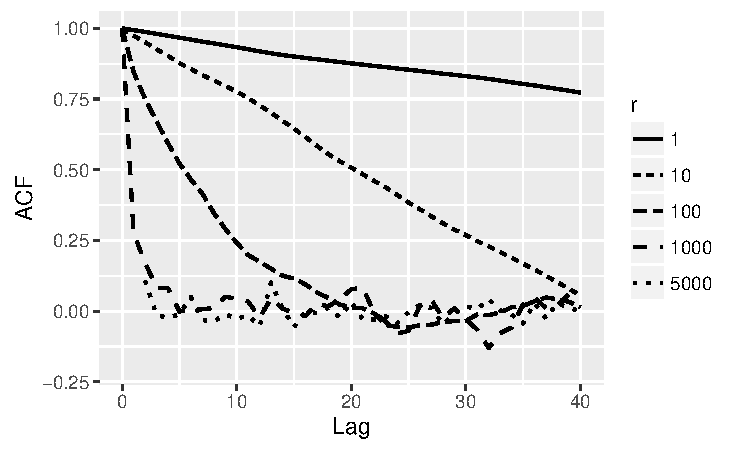
\includegraphics[width=1\textwidth]{probit_demo_acf_prop.pdf}
  \caption{Autocorrelation function (ACF) illustrating the effects of the variance increase of $r$ on improving the mixing of the proposal distribution $\beta^*$.}
 \label{probit_demo_intercept_proposal}
\end{subfigure}
  \hfill
   \begin{subfigure}[b]{0.49\textwidth}
 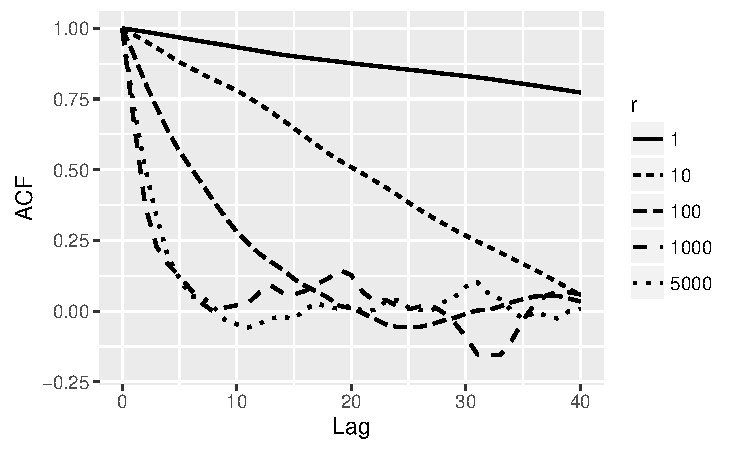
\includegraphics[width=1\textwidth]{probit_demo_acf.pdf}
  \caption{ACF illustrating the mixing of the posterior sample $\beta$ after using Metropolis-Hastings step to accept the proposal from the calibrated distribution.}
   \label{probit_demo_intercept_posteriorsample}
\end{subfigure}
 \caption{Panel (a) demonstrates the adjustment of the step size via increasing the conditional variance in the proposal $\beta^*$ and panel (b) shows its effect after the proposal from the calibrated distribution is accepted as $\beta$ into the Markov chain by the M-H criterion.}
 \label{probit_demo_intercept}
 \end{figure}


\subsection{Adaptation of $r$ and $b$}
The chosen value for $r$ and $b$ are important to ensure good calibration and sufficiently large acceptance rate. Intercept-only probit is a special case where it is possible to estimate the high posterior density region, hence select $b$ and $r$ before sampling. To apply CDA more broadly, we need to be able to handle cases where this is not possible. In this section, we develop a strategy for adaptation of $r$ and $b$. After the acceptance rate reaches a pre-set threshold, we stop adapting and collect the posterior sample.

In the adapting period, we start from an moderately large value for all $r_i$. And  $r_i$ is bounded in the region of $[1, \kappa]$, where the lower bound $1$ corresponds to no adjustment and $\kappa$ is a maximal value set to prevent numeric error. As the lower bound of the acceptance probability in \eqref{eq:mh-criterion} is the product of  $\alpha_i= \frac{   L_r(\xbeta;y_i) L(\xbeta^*;y_i)}{ L_r(\xbeta^*;y_i)L(\xbeta;y_i) }$ over all $i$. When $\alpha_i<1$, we decrease $r_i$ to reduce the step size; when $\alpha_i>1$, we increase $r_i$ to raise the step size.  As an empirical value, we multiply $r_i$ by $\sqrt \alpha_i$ at the end of each iteration. In the meantime, we set $b_i= \xbeta (\sqrt{r_i}-1)$ as it minimizes the difference between $\Phi( \frac{\xbeta+b_i}{\sqrt{r_i}})$ and $\Phi(\xbeta)$.

The acceptance rate is calculated as the total count of acceptance divided by the adapting iterations taken thus far. After it reaches satisfactory level (e.g. $0.3$), we stop the adaption and keep $r$ and $b$ fixed. The posterior is collected as ordinary Metropolis-Hastings sampling.

To illustrate the case where $r$ and $b$ are difficult to pre-set, we consider a probit regression with an intercept and two predictors $x_{i,1},x_{i,2}\sim \No(1,1)$, with $\beta=\{-5,1,-1\}'$, generating $20$ positive outcomes among $n=10,000$. 

In this testing case, the \cite{albert1993bayesian} DA algorithm suffers from extremely slow mixing (Figure~\ref{probit_reg_trace} and \ref{probit_reg_acf}). To compare with an early method, we tested the parameter expansion algorithm (PX-DA) proposed by \cite{liu1999parameter}. PX-DA only mildly reduces the correlation, as it does not solve the variance mismatch problem.

To calibrate, we apply CDA with initial value of $200$ for all $r_i$ and use the adaptive algorithm for 100 iterations, obtaining an acceptance rate of $0.36$. We use the fixed $r$ and $b$ to collect the posterior sample. The calibrated algorithm leads to significant improvement of the mixing.

It is interesting to note relation between the adapted $r_i$ and the posterior value of $\xbeta$ (Figure~\ref{probit_reg_r}). The very negative $\xbeta$ ($< -2$) suffers the mis-match in the conditional and marginal variance, hence allows large $r_i$ to adjust the step size. The bias reducing term $b_i$ is linear in $(\sqrt{r_i}-1 ) \xbeta$ as expected (Figure~\ref{probit_reg_b}).
 
 
\begin{figure}[H]
 % \centering
  \begin{subfigure}[b]{0.49\textwidth}
 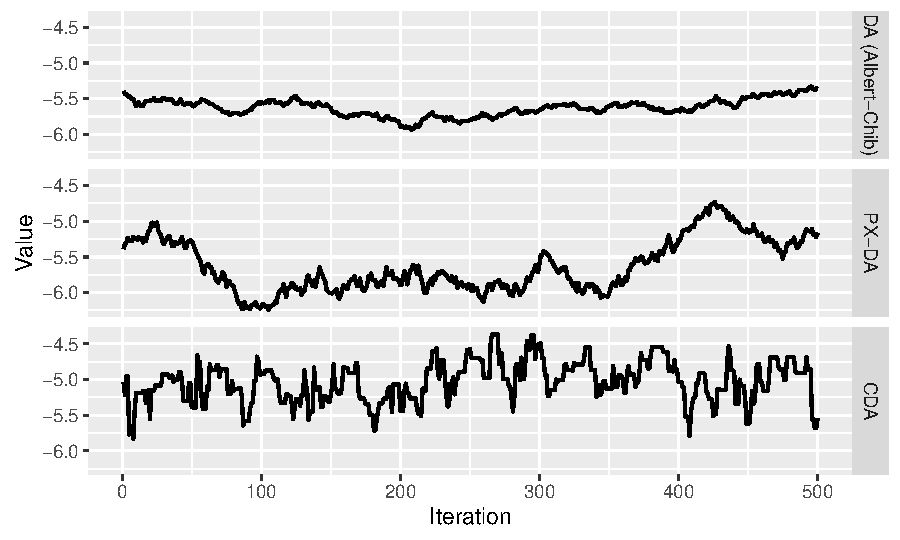
\includegraphics[width=1\textwidth]{probit15_trace_plot.pdf}
  \caption{Traceplot illustrating mixing performance of the original DA, parameter expanded DA and CDA algorithms in probit regression with rare event data.}
  \label{probit_reg_trace}
\end{subfigure}
  \hfill
   \begin{subfigure}[b]{0.49\textwidth}
 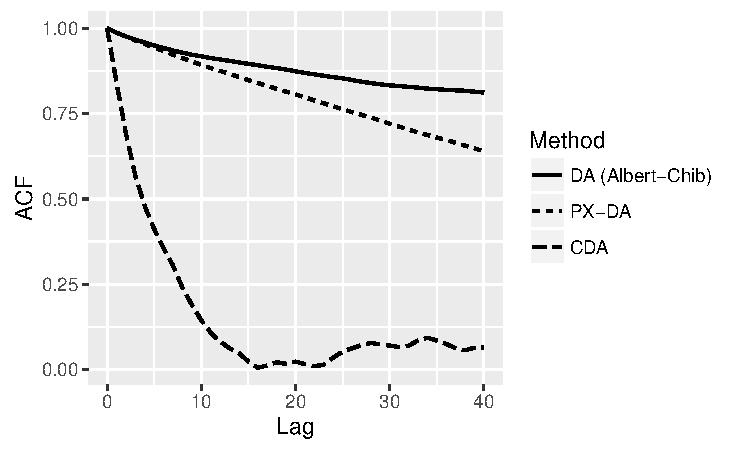
\includegraphics[width=1\textwidth]{probit15_acf.pdf}
  \caption{Autocorrelation function (ACF) illustrating the slow mixing of the DA and parameter expanded DA in rare event data, and CDA correcting this problem.}
    \label{probit_reg_acf}
\end{subfigure}
   \begin{subfigure}[b]{0.49\textwidth}
 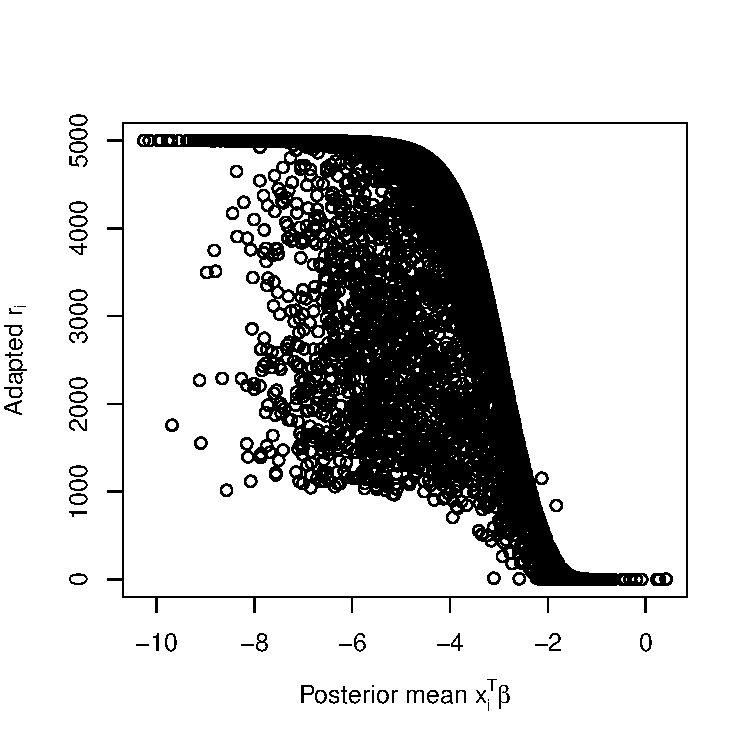
\includegraphics[width=1\textwidth]{probit_cda_r}
  \caption{Numerically adapted $r_i$ showing the room for variance increase is related to the  value of $|\xbeta|$.}
    \label{probit_reg_r}
\end{subfigure}
  \begin{subfigure}[b]{0.49\textwidth}
 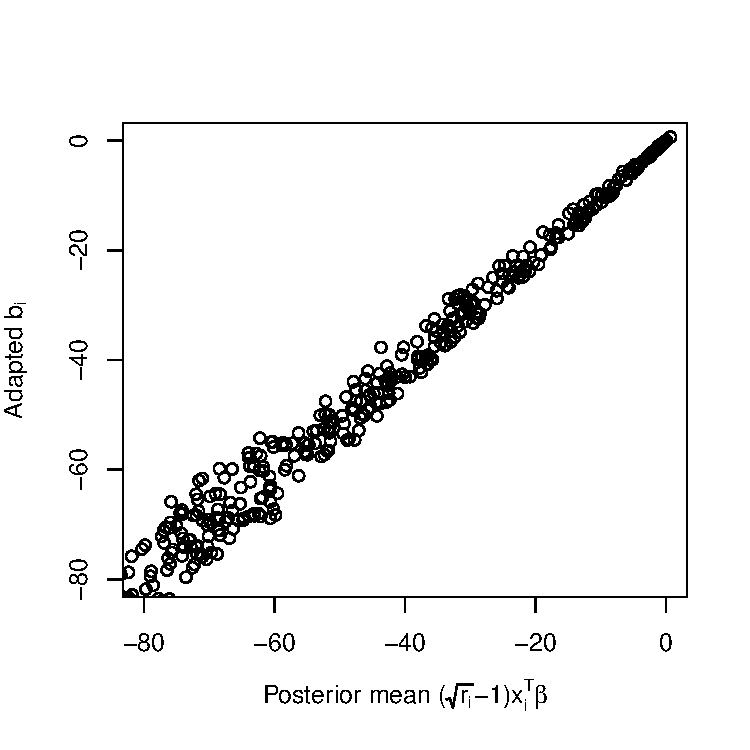
\includegraphics[width=1\textwidth]{probit_cda_b}
  \caption{Numerically adapted $b_i$ learned during the tuning period is close to $(1-\sqrt{r_i} ) \xbeta$ based on the posterior mean.}
      \label{probit_reg_b}
\end{subfigure}
 \caption{Panel (a) demonstrates in traceplot and panel (b) in autocorrelation about the substantial improvement in CDA by correcting the variance mis-match in probit regression with rare event data, compared with the original \citep{albert1993bayesian} and parameter-expanded methods \citep{liu1999parameter}. Panel (c) shows the room for the variance increase in $r_i$ ($r_i=1$: no increase) with respect to the value of $\xbeta$. Panel (d) shows the adapted bias reducing term is close to the true bias based on the posterior mean.}
 \end{figure}

\subsection{Controlling Latent Variable in Conditional Variance}

The success of CDA relies on the fact that the calibrated conditional with increased variance can still yield the similar marginal form as the original. Using $\pi(\theta|y)=\int\pi(\theta|z,y)\pi(z|y) dz$, when $\mbox{cov}(\theta|z,y)$ does not involve the latent variable $z$ (like in the probit example), the multiplication with $r$ does not affect the integrability. Otherwise, when $z$ is part of the variance, multiply $r$ directly on the conditional variance might make the integration difficult. To solve this issue, one can influence the value of $z$ by modifying $\pi(z|y)$ instead, while still maintain the closed-form marginal.

To illustrate, consider the logistic regression:

\be
y_i \sim \Bern(p_i), \quad p_i = \frac{\exp(x_i \beta)}{1+\exp(x_i \beta)},
\ee
and improper prior $\pi(\beta)=1$. The Polya-Gamma data augmentation has the update rule \citep{polson2013bayesian}:

\be
 z_i &\sim {\PG}(1, |\xbeta|),\\
\beta &\sim \No \left(  (X' Z X)^{-1}   X'  (y-\frac{1}{2})  ,  (X' Z X)^{-1}  \right),
\ee
where $Z= diag(z_1,\ldots,z_n)$. This is due to the integration $L(y_i \mid \xbeta)=  \int \exp\{ \xbeta (y_i-1/2)\} \exp(-\frac{z_i (\xbeta)^2}{2}) \PG(z_i \mid 1,0) dz_i$. As described above, the direct multiplying $r_i$ to $z_i$ would make it difficult to integrate over $z$.

Observing the value of $z$ is influenced by the first parameter in Polya-Gamma, we modify $\PG(z_i \mid 1,0)$ by replacing $1$ with the auxiliary parameter $r_i$. This calibration does not affect the integrability, applying bias correction term $b_i$ on $\xbeta$, leading to:


\be
L_r(\xbeta;y_i) = & \int_{0}^{\infty}  \exp\{ (\xbeta+b_i) (y_i-r_i/2)\} \exp(-\frac{z_i (\xbeta+b_i)^2}{2}) \PG(z_i \mid r_i,0) dz_i \\
= &  \frac{\exp \{ (x_i \beta + b_i)y_i \}}{\{1+\exp(\xbeta +b_i)\}^{r_i}},
\label{eq:prop-marginal-logit}
\ee
yielding the update rule for the proposal:

\be
 z_i &\sim {\PG}(r_i, |\xbeta+b_i|),\\
\beta^* &\sim \No \left(  (X' Z X)^{-1}  X'  (y -r_i/2- Zb) ,  (X' Z X)^{-1}  \right),
\ee

Unlike the probit example where the variance increase is deterministic, the step size tuning here is stochastic: utilizing $\bb{E}z_i= \frac{r_i}{2 (|\xbeta+b_i|)}\tanh(\frac{|\xbeta+b_i|}{2})$ and $\bb{E}z_i^{-1}= \int_0^{\infty} \prod_{k=1}^{\infty} (1+ d_k^{-1} t) ^{-r_i} dt$ with $d_k=2(k-\frac{1}{2})^2\pi^2 + \frac{(x_i\beta+b_i)^2}{2}$ (combining results from \cite{cressie1981moment} and \cite{polson2013bayesian}), with smaller $r_i$, $z_i^{-1}$ will have larger value with high probability, leading to large variance in $(X' Z X)^{-1}$.

Similar to probit example, M-H step can be derived to accept the proposal $\beta^*$:

\be
1 \wedge  \frac{  \prod_i L_r(\xbeta;y_i) L(\xbeta^*;y_i)}{\prod_i  L_r(\xbeta^*;y_i)L(\xbeta;y_i) },
\ee

where $L(\theta;y_i)=\frac{\exp(\theta y_i)}{1+\exp(\theta)}$. It then can derived the adaptive form for $b_i$ should be $\log[  \{1+\exp(\xbeta)\}^{1/r_i} -1] - \xbeta$. 


For illustration, we use a two parameter intercept-slope model with $x_1\sim \No(0,1)$ and $\beta=\{-9,1\}$. With $n= 10^5$, it leads to rare positive outcome $\sum y_{i} = 50 $. We adapt the $r$ and $b$ for $100$ steps, reaching acceptance rate of $0.9$; then stopp adaption and collect the posterior sample. The different mixing performances in the original DA and the calibrated one are shown in Figure~\ref{logit_random_mixing}.


\begin{figure}[H]
 % \centering
  \begin{subfigure}[b]{0.49\textwidth}
 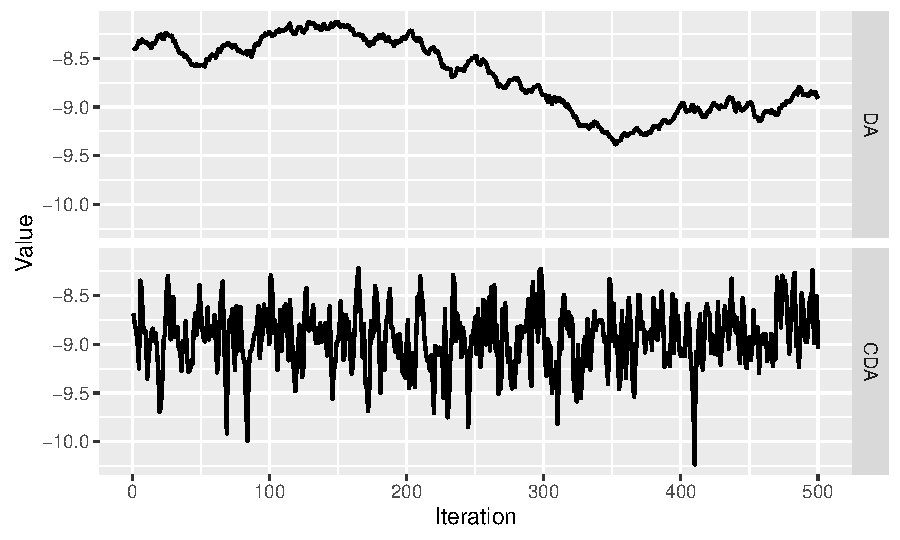
\includegraphics[width=1\textwidth]{logit_random_trace_plot.pdf}
  \caption{Traceplot illustrating mixing performance of the original DA and CDA algorithms in logistic regression.}
\end{subfigure}
  \hfill
   \begin{subfigure}[b]{0.49\textwidth}
 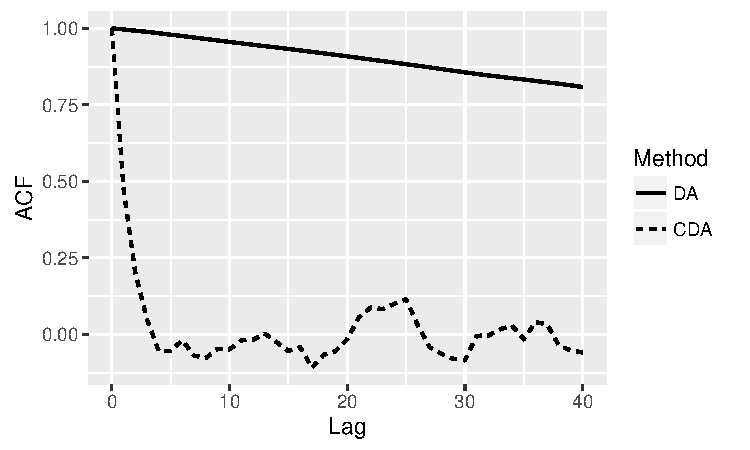
\includegraphics[width=1\textwidth]{logit_random_acf.pdf}
  \caption{Autocorrelation function (ACF) illustrating the different performances of the DA and CDA.}
\end{subfigure}
 \caption{Panel (a) demonstrates in traceplot and panel (b) in autocorrelation about the substantial improvement in CDA by correcting the variance mis-match in logistic regression with rare event data, compared with the original \citep{polson2013bayesian}.}
    \label{logit_random_mixing}
 \end{figure}



\subsection{General Algorithm}

Before proceeding into theory, we summarize the general algorithm for CDA. We assume the parameters are multi-dimensional and can be divided into two groups $\{ \theta, \eta\}$, where only $\theta$ are the ones suffering from slow mixing. With Gibbs sampling, we alternatively sample $\eta\mid\theta, y$ and $\theta\mid \eta,y$. To calibrate, we now focus on $\theta\mid \eta,y$ and omit $\eta$ for notational ease. Breaking down the likelihood into the product of the augmented likelihoods, each has:

\be \label{eq:da_decomposition}
L(m_i(\theta);y_i) = C\int \pi\left(m_i(\theta)|z_i,y_i \right)\pi(z_i|y_i) d z_i
\ee
where $C$ is the constant free from $\theta$, $m_i(\theta)$ is the function $m_i:\bb R^p \mapsto \bb R$. For example, $m_i (\beta) = x_i\beta$ in regression. Let the the conditional distribution for $\theta$ be:

\be
\theta \mid z,y &\sim f(\mu,\Sigma).
\ee
We adjust $\Sigma$ with the auxiliary parameter $r_i$: if $\Sigma$ is free from $z$, we multiply $r_i$ into $\pi\left(m_i(\theta)|z_i,y_i \right)$ like the probit example; otherwise, we change the parameters in $\pi(z_i|y_i)$ to influence the value of $z_i$ like the logit example. With an additional parameter $b_i$ to reduce the bias, we obtain the calibrated data augmentation:

\be \label{eq:cda_decomposition}
L_r(m_i(\theta) ; y_i) = C_r\int \pi_r\left(m_i(\theta)+b_i|z_i,y_i \right)\pi_r(z_i|y_i) d z_i
\ee

Then the proposal update rule can be formed:

\be
z_i & \sim \pi(z_i| m_i(\theta)+b_i) \\
\theta^* &\sim f(\mu(m_i(\theta)+b_i, z),\Sigma(z)).
\ee
and accepting new $\theta^*$ with probability:
\be
1 \wedge \prod_i \alpha_i, \quad \alpha_i = \frac{L(m_i(\theta^*); y_i) L_r(m_i(\theta) ; y_i)} {L(m_i(\theta); y_i) L_r(m_i(\theta^*); y_i)}.
\label{eq:mh-criterion}
\ee

To increase the acceptance rate, we adaptively tune $r$ and $b$ until the the acceptance rate reaches the preset threshold (e.g. $0.3$). We start from an $r_i$ that corresponds to moderate increase in the step size. Then at the end of each iteration, increase or decrease $r_i$ based on $\alpha_i>1$ or $\alpha_i<1$ (assuming smaller $r_i$ has larger chance of $\alpha_i>1$). After the adaptation, we fix $r$ and $b$ and collect the posterior samples.

% Skip the always adapting parameter scheme.
%\subsection{Special Case without Metropolis-Hastings}
%
%In some cases, if the distance between the proposal $\pi^{*}(f_i(\theta)+b_i \mid y_i, r_i)$ and original $\pi(f_i(\theta)\mid y_i)$ can be strictly bounded, the Metropolis-Hastings step can be skipped, directly accepting $\theta^*$. This generates an approximate Gibbs sampler, a non-reversible Markov chain with a modified target distribution. But since the error is non-noticeable, it can be used as a good and fast approximate to the original slow algorithm.
%
%Taking the logit CDA as an example, note the value for $b_i$ to correct the difference would be $\log[  \{1+\exp(\xbeta)\}^{1/r_i} -1] - \xbeta$. Its expansion yields $\log\{ 1/r_{i} + \frac{1/r_{i}(1/r_{i}-1)}{2!} \exp(\xbeta)+ \frac{1/r_{i}(1/r_{i}-1)(1/r_{i}-2)}{3!} \exp(2\xbeta) +\ldots \ \}$. The suggests when $\exp(\xbeta)$ is close to $0$, $b_i \approx -\log r_{i}$. Then the bound can be calculated between the marginal likelihoods based on the original and calibrated form. We postpone the details of total variation distance to the next section.
%
%This simplifies the update rule to:
%
%\be
% z_i &\sim {\PG}(r_i, |\xbeta - \log r_i|),\\
%\beta &\sim \No \left(  (X' Z X)^{-1}  X'  (y -r_i/2- Z \log r) ,  (X' Z X)^{-1}, \right)
%\ee
%where $r_i$ is taking a small value when $\exp(\xbeta) < \eta$, otherwise $r_i=1$. 
%
%As the posterior are directly generated from the approximate, the bound needs to be carefully controlled via $r_i$. Therefore, instead of  being fixed after the tuning as in the general case, $r_i$ is used adaptively throughout the sampling. This would cause convergence issue; however, choosing $r_{i} = \sup[\tau{\exp(2\xbeta)}  \vee {\exp(\xbeta)} ]  \wedge 1$ ($\tau>1$) as the maximal function of posterior samples leads to a diminishing adaptation scenario: the probability of $r_i$ changing converges to $0$ hence the difference in two consecutive transition kernels diminishes,  ensuring the convergence of the chain \citep{roberts2007coupling}.
% 

\section{Theory: Mixing Acceleration}

The mixing of Markov chain can be described by the geometric convergence rate. Let $\mathcal{P}(\theta,.)$ be the the Markov transition measure and $\pi(.)$ be the target invariant measure and $\theta$ be the state in the state space $\varTheta$. Starting from the initial state $\theta^{(0)}$, the chain is geometrically ergodic if there exist $M: \varTheta \rightarrow [0, \infty)$ and $\rho\in[0,1)$ such that $||\mathcal{P}^k(\theta,.)-\pi(.) ||_{TV} \le M(\theta^{(0)}) \rho^k$, where $||.||_{TV}$ is the total variation distance $|| P_1 -P_2 ||_{TV} = \underset{\mathcal A\in \mathcal F}\sup ||P_1(\mathcal A)-P_2(\mathcal A)||$. As the number of iterations $k\rightarrow \infty$, $||\mathcal{P}^k(\theta,.)-\pi(.) ||_{TV} \rightarrow 0$ leading to convergence to the target. The slow mixing is attributed to $\rho$ being too close to $1$. As shown by \citep{scott2016bayes}, the $\rho$ approaches $1$ as $n$ increases, leading to a complete break-down of algorithm. Therefore, we study how the calibration can solve this problem.

We first utilize another related quantity, the norm of the forward operator $||\bf{F}||$, defined as  ${\bf F}s(\theta)=\int \mathcal{P}(\theta,\theta') s(\theta') d\theta' = E\{ s(\theta') | \theta \}$. In a Hilbert space $L^2(\pi)=\{s(\theta): \bb E s(\theta)=0, \mbox{var}\{s(\theta)\}<\infty \}$, the norm is defined as the maximal correlation between two states $||{\bf F}||=\underset{s(\theta),t(\theta)\in L^2(\pi)}{\sup}\;\mbox{corr}(s(\theta),t(\theta^{'}))$ \citep{liu2008monte}. This norm is related to $\rho$: when the chain is reversible with detailed balance (e.g. M-H), $\lim_{k\rightarrow \infty}||{\bf F}^k||^{1/k}=\rho$; when the chain is non-reversible, $||{\bf F}||^2$ is equal to the convergence rate of the reversibilized chain \citep{fill1991eigenvalue}.

The original DA samples in the sequence of $\theta' \rightarrow z' \rightarrow \theta \rightarrow z$. Omitting $y$ for simpler notation, by Lemma 4 in \cite{liu1994collapsed}:

\be
||{\bf F}_{DA}|| =\underset{s(\theta)\in L^2(\pi)}{\sup}\; \frac{\mbox{var}_{DA} [ \bb E_{DA} \{ s(\theta,z)|\theta^{'},z'\}]}{\mbox{var}_{DA}\{s(\theta,z) \} }  & = \underset{s(\theta)\in L^2(\pi)}{\sup}\; \frac{\mbox{var}_{DA} [ \bb E_{DA} \{ s(\theta)|z'\}]}{\mbox{var}_{DA}\{s(\theta) \} } \\
& = 1- \underset{s(\theta)\in L^2(\pi)}{\inf}\; \frac{\bb E_{DA}  [  \mbox{var}_{DA}\{ s(\theta)|z'\}]}{\mbox{var}_{DA}\{s(\theta) \} } 
\label{eq:norm_da}
\ee

The slow mixing is obviously due to ${\bb E_{DA}  [  \mbox{var}_{DA}\{ s(\theta)|z'\}]} \ll {\mbox{var}_{DA}\{s(\theta) \} }$.

The calibrated DA is slightly different, by proposing $\theta^*$ in the calibrated sample and use Metropolis-Hastings to accept the new state $\beta^*$ or keep the previous state $\beta$, it in fact samples in the sequence of $( \theta' , z' )\rightarrow \theta \rightarrow z$, similarly we obtain:

\be
||{\bf F}_{CDA}|| =\underset{s(\theta)\in L^2(\pi)}{\sup}\; \frac{\mbox{var}_{CDA} [ \bb E_{CDA} \{ s(\theta,z)|\theta^{'},z'\}]}{\mbox{var}_{CDA}\{s(\theta,z) \} }  = 1- \underset{s(\theta)\in L^2(\pi)}{\inf}\; \frac{\bb E _{CDA} [  \mbox{var}_{CDA}\{ s(\theta)|z',\theta'\}]}{\mbox{var}_{CDA}\{s(\theta) \} } 
\label{eq:norm_cda}
\ee


To compare the \eqref{eq:norm_da} and \eqref{eq:norm_cda} directly, we rely on the following lemma.

\begin{lemma}
	In Metropolis-Hastings step with current state $\theta'$ and proposal state $\theta^*$ from $f(\theta^*; z')$, if the acceptance probability $p\ge p_0$, the generated state $\theta$ satisfies $\mbox{var}_{CDA}\{ s(\theta)|z', \theta'\} \ge   p_0\cdot \mbox{var}_{CDA} (s(\theta^*)|z')$.
\end{lemma}

Therefore, we can induce an increase in $\bb E [\mbox{var}\{ s(\theta)|z'\}]$ by $\gamma$ times, and obtain the following acceleration:

\begin{theorem}
Let ${\bf F}_{DA}$ and ${\bf F}_{CDA}$ be the forward operators corresponding to the standard DA and the calibrated DA; $\theta$ be the random variable from the DA updating rule and $\theta^*$ be the one from the CDA proposal. Assume the conditional variance increase in the CDA proposal has ${  \bb E [\mbox {var}_{CDA}\{ s(\theta^*)|z,y\}]  } \ge \gamma \cdot { \bb E [\mbox {var}_{DA}\{ s(\theta)|z,y\}]}$ with the Metropolis-Hastings acceptance probability in \eqref{eq:mh-criterion} greater or equal to $p_0>0$. Then if $p_0 \gamma \ge 1$, 
$$||{\bf F}_{CDA}||\le 1- \gamma p_0 \cdot \underset{s(\theta)\in L^2(\pi)}{\inf}\; \frac{\bb E_{DA}  [  \mbox{var}_{DA}\{ s(\theta)|z'\}]}{\mbox{var}_{DA}\{s(\theta) \} } 
\le ||{\bf F}_{DA}||.$$
\end{theorem}

%In practice, $\underset{k=1\ldots p}{\sup}\;\mbox{corr}(\theta_k,\theta^{'}_k) $ is often used as a more tractable approximate to $||\bf F||$. In the probit example, since $z$ is not in the conditional variance, direct increase of $r$ in $\bb E [\mbox {var}_{CDA}\{ s(\theta)|z,y\}] =(X'R^{-1}X)^{-1}$ leads to mixing acceleration. In the logit example, the increase in $\bb E [\mbox {var}_{CDA}\{ s(\theta)|z,y\}] =\bb E(X'ZX)^{-1}$ can be numerically evaluated  (see section 2.2).

As the result, with an increase in $\gamma$ by raising the conditional variance, and a $p_0$ away from $0$, one can significantly accelerate the mixing. The large $p_0$ is attributed to the similarity between $L_r$ and $L$ in \eqref{eq:mh-criterion}, as the result of adaptation. For example, in the logit CDA:

\be
\alpha_i = \frac{ \{1+\exp(\xbeta)\}   \{1+\exp(\xbeta^*+b_i)\}^{r_i} } {  \{1+\exp(\xbeta^*)\}  \{1+\exp(\xbeta+b_i)\}^{r_i}    } 
\ee
when $\xbeta$ is negative (corresponding to large variance gap that causes slow mixing), the adapted bias reduction term $b_i  = \log\{ 1/r_{i} + O (\frac{\exp(\xbeta)}{r_i} )\} \approx -\log r_i$. Then $\{ 1+\exp(\xbeta-\log r_i)\}^{r_i} = 1+\exp(\xbeta) + O(\frac{\exp(2\xbeta) }{r_i})$.


\section{Real Data Application: Poisson Regression for Online Advertisement Tracking}

We now apply CDA to a real data application in online advertisement tracking. The advertisement is displayed on $n=59,792$ originating websites, pointing to $96$ different targets. The count of click-throughs is recorded for each combination. The counts contain many zeros ($95.5\%$), as not all $96$ advertisements are shown on all the websites. For commercial interests, it is useful  to predict the traffic of the new advertisements using the existing ones. Therefore, we use the data of $95$ advertisements as predictors $x_i$ and the one left as the outcome $y_i$ for a count regression. We use training data collected from a two-week period, and a validation data set collected during another two-week window. 

One common practice to handle the large proportion of zeros is to use zero-inflated Poisson. However, for predictive modeling, this is suboptimal as it would require another set of coefficients to predict the latent binary event, e.g. $y_i\sim p\left( g(x_i\eta)\right)  \delta_0+ \{ 1-p\left( g(x_i \eta) \right) \} Poisson\{\exp (x_i \beta)\}$. Instead, it is rather useful to consider a simpler model  $y_i\sim Poisson\{\exp(\beta_0+ \sum_j x_{i,j}\beta_j)\}$ with a quite negative intercept $\beta_0$.

It is known that the posterior sampling for Poisson is hindered by slow mixing, which is especially worse with large amount of zeros. The traditional M-H lacks a good strategy to propose multidimensional variables ($p=96$ in this case). There is a Gibbs sampling strategy, first discovered by \citep{zhou2012lognormal} with negative binomial approximation. We further simplify and present the algorithm.

The Poisson density can be viewed as a limit:
\be
L(\xbeta;y)=\frac{ \exp(y_i \xbeta)}{\exp\{\exp(\xbeta)\}y!} =\lim_{\lambda\rightarrow\infty}\frac{\exp(y_i \xbeta)}{\{1+ \exp(\xbeta)/\lambda\}^{\lambda}y!}.
\ee

With large but finite $\lambda$ (e.g. $10,000$), one can sample from the approximate posterior:

\be
z_i \sim & \PG\left (\lambda, \xbeta -\log \lambda\right)\\
\beta \sim & \No \left( \big[ (X' ZX )^{-1} X'  \big ( y - \lambda/2 + z \log \lambda \big) ,(X' Z X )^{-1} \right)
\ee

The problem with this DA is that as $\lambda$ increases, the large $z$ quickly reduces the conditional variance for $\beta$, creating mixing bottleneck. It inevitably becomes a dilemma to trade between accuracy or mixing rate in choosing $\lambda$.

As $\lambda$ control the magnitude of the latent $z$, the calibration is straightforward by replacing $\lambda$ with small $r_i$ and $-\log \lambda$ with $b_i$, giving the calibrated likelihood:

\be
L_r(\xbeta;y)=\frac{\exp \{ y_i (\xbeta + b_i)\}}{\{1+ \exp (\xbeta + b_i)\}^{r_i}},
\ee
which generates the same sampling algorithm as the CDA in logit regression, except that $r_i>y_i$ to ensure the posterior properiety.

We run the approximate DA with large $\lambda=10,000$ and the exact CDA for posterior computation. For CDA, we adapt for $100$ iterations and reaches an acceptance rate of $0.6$. We then run each algorithm for $4,000$ steps and use the last $1,000$ as the posterior sample.

The mixing of DA and CDA is compared in traceplots and autocorrelation plots in Figure~\ref{data_poisson}. DA shows slow mixing for several parameters (Figure\ref{acf_poi_da}), including the important intercept estimate $\beta_0$ (first plot in Figure\ref{traceplot_poi_da}). After calibration, the slow mixing problem is solved:  {\it all} of 96 parameters show very low autocorrelation.

 \begin{figure}[H]
 % \centering
   \begin{subfigure}[b]{0.45\textwidth}
 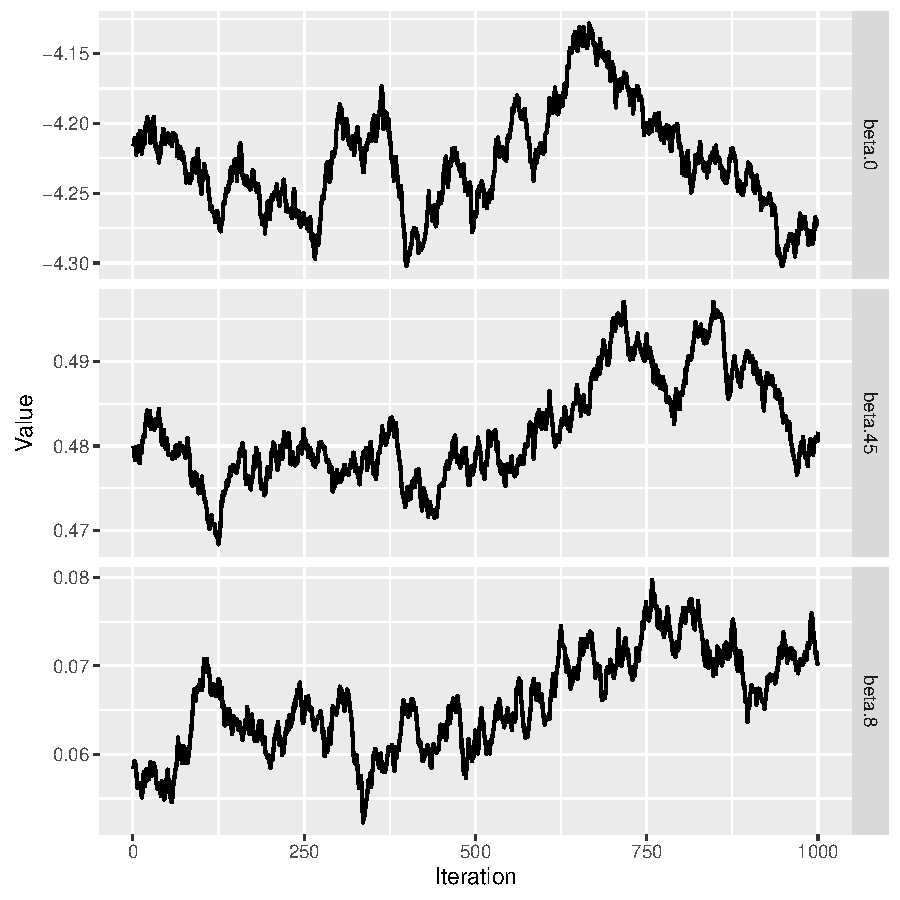
\includegraphics[width=1\textwidth]{traceplot_poisson_da}
 \caption{Trace plots of three parameters from DA.}
  \label{traceplot_poi_da}
 \end{subfigure}
  \hfill 
 \begin{subfigure}[b]{0.45\textwidth}
 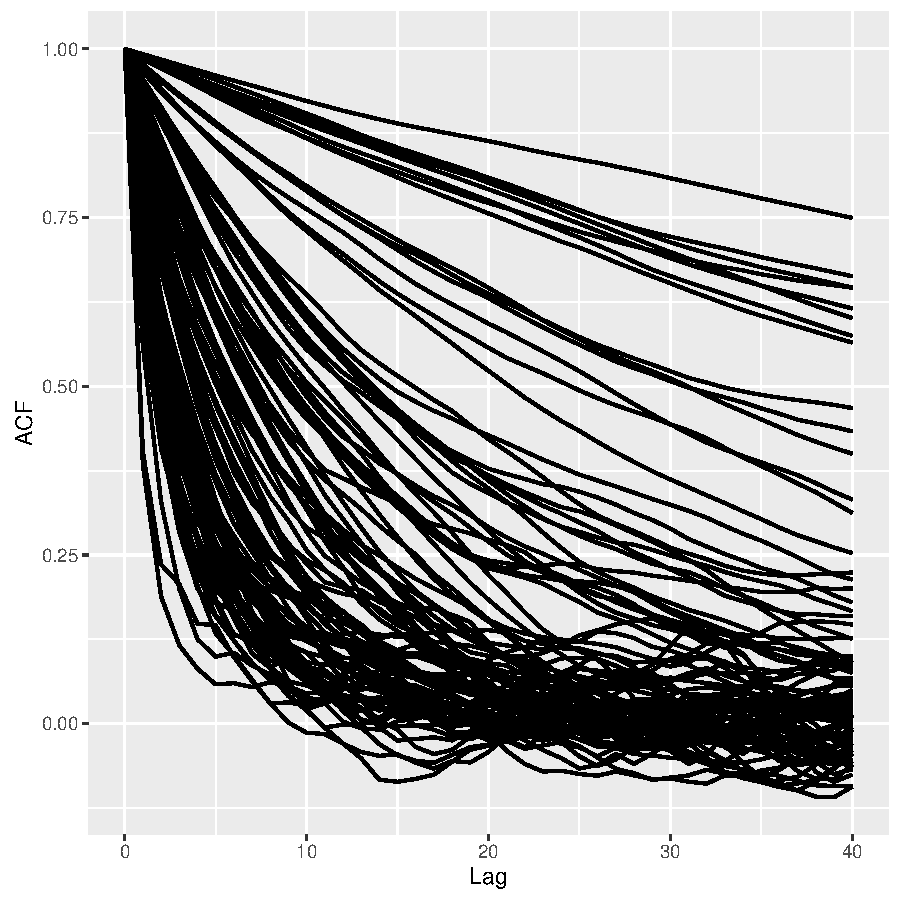
\includegraphics[width=1\textwidth]{poisson_da_acf.pdf}
 \caption{Autocorrelation of all the 96 $\beta$'s from DA.}
   \label{acf_poi_da}
 \end{subfigure} 
  \begin{subfigure}[b]{0.45\textwidth}
 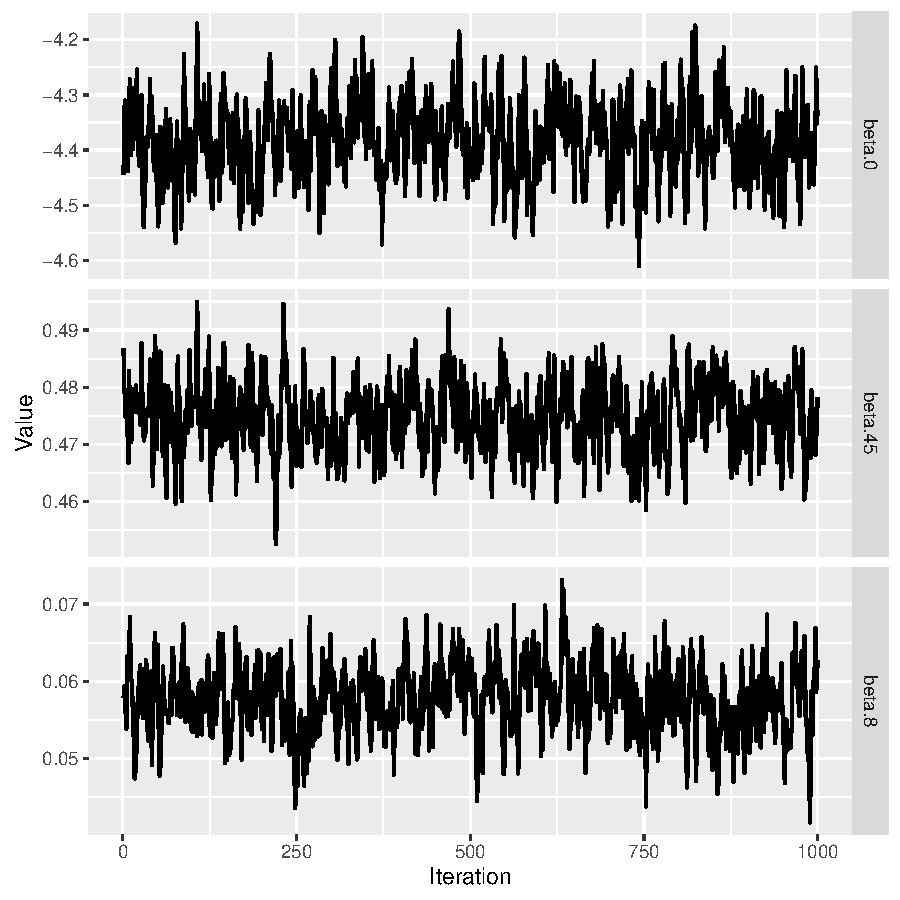
\includegraphics[width=1\textwidth]{traceplot_poisson_cda}
 \caption{Trace plots of three parameters from CDA.}
  \label{traceplot_poi_ada}
 \end{subfigure}
  \hfill 
 \begin{subfigure}[b]{0.45\textwidth}
 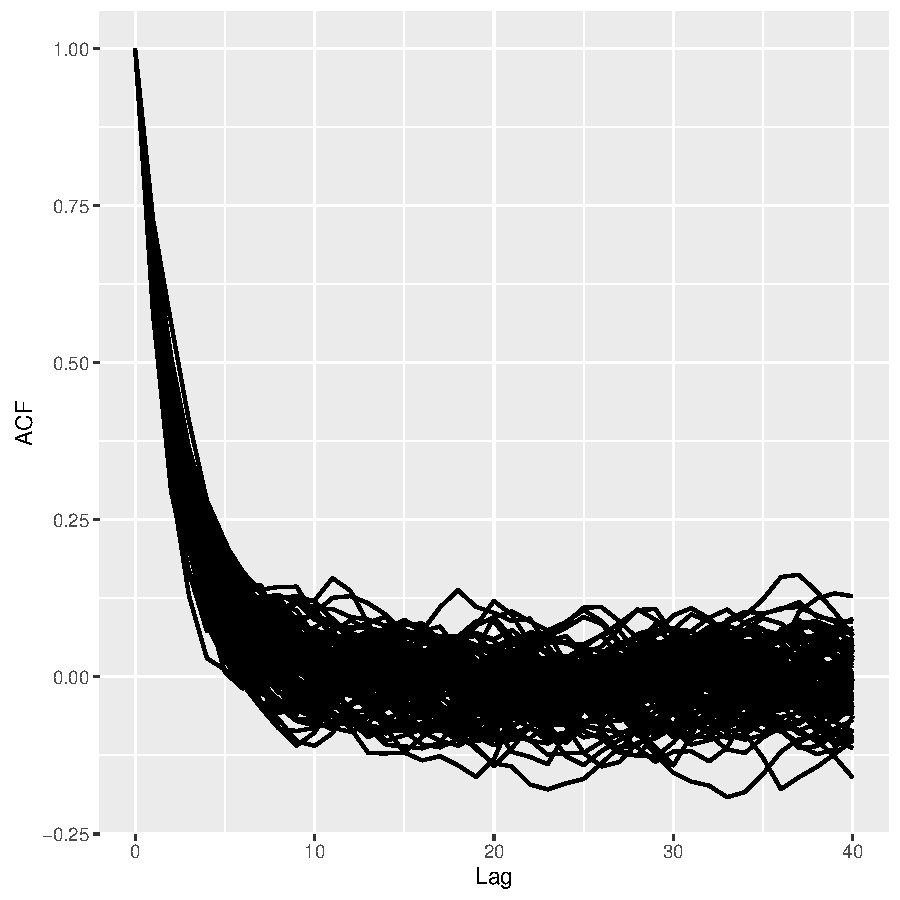
\includegraphics[width=1\textwidth]{poisson_cda_acf.pdf}
 \caption{Autocorrelation of all the 96 $\beta$'s from CDA.}
   \label{acf_poi_ada}
 \end{subfigure}
 \caption{Panels (c) and (d) show significant improvement of the mixing in Poisson data augmentation. Panel (d) show the CDA reduces the autocorrelation for all of the parameters.}
 \label{data_poisson}
 \end{figure}


To empirically evaluate the accuracy of the estimates, we also run Hamiltonian Monte Carlo (HMC) as the reference. HMC is known for its good mixing properties, despite of its costly evaluation. We list the parameter estimates and fit statistics in Table~\ref{table:Poisson}. For simplicity, we include the posterior mean and standard deviation for the intercept $\beta_0$ and the norm of the coefficients $\sum_{j=0}^{95} |\beta_j|$. For goodness-of-fit, we compute root-mean-squared error $RMSE= \sqrt{ \sum_{i=1}^n  (y_i-\mu_i)^2/n}$ and the deviance $D=2\sum_{i=1}^n \{ y_i \log(y_i/\mu_i) -(y_i-\mu_i)\}$, with $\mu_i=\exp( x_i{\hat\beta})$ and ${\hat\beta}$ as the posterior mean. For prediction performance, we use the testing dataset and $\hat y_{i,new}=\exp( x_{i,new}{\hat\beta})$ as the estimator. We evaluate the cross-validation RMSE between $y_{i,new}$ and $\hat y_{i,new}$.

As expected, the estimates for $\beta_0$ from all models are quite negative. However, the DA severely underestimates the variance of the intercept. The coefficient norm also differs greatly from CDA and HMC. Obviously, the poor mixing causes the Markov chain in DA to be trapped in a suboptimal state. After calibration, CDA performs exceptionally well in fit statistics and the validation error that is almost $4$ times lower. The results of CDA and HMC are nearly identical (see appendix for more comparison).

Lastly, it is worth to compare the computing time needed for the three methods. The CDA operates at almost the same cost as the original DA in each iteration. After the extra adaptation period (about $100$ iterations), CDA quickly converges to the target in the first few iterations; whereas DA seems to be stuck even after $2,000$ iterations. HMC is computationally intensive as it requires evaluation of the gradient and multiple Hamiltonian steps in generating a proposal, therefore the speed is about $10$ times slower; and the adaptation in both step size and step number is also time-consuming. In conclusion, CDA is most computationally efficient.


\begin{table}[H]
\centering
\begin{tabular}{|l |r |r| r| r |} 
 \hline
                          & DA & CDA & HMC\\
 [0.5ex]
 \hline
$\beta_0$                         & -4.21 (0.042)& -4.38 (0.075) & -4.47 (0.071) \\
$\sum_{j=0}^{95} |\beta_j|$         & 12.24 (0.10)&  8.58 (0.11)  & 8.68 (0.11)  \\
RMSE                              & 32.86        & 5.06          & 4.88\\
D                                 & 182127.7     & 107076.9      & 106791.3\\
CV-RMSE                           & 32.01        & 8.61          & 8.28\\
Steps for Adaptation \& Burn-in                & 2000         & 100            & 500 \\
Computing Speed (per 1,000 steps)  & 25 mins       & 26 mins        & 300 mins\\
 \hline
\end{tabular}
\caption{Performance of DA, CDA and HMC in Poisson log-linear regression with online advertisement tracking data. Posterior estimates for the intercept and the norm of the coefficients are shown. The CDA shows much improved fit statistics such as root-mean-squared error (RMSE) and deviance (D). In cross-validation (CV-RMSE), the CDA outperforms DA in nearly $4$ times lower in error. The CDA converges much more rapidly than DA. CDA agrees with the HMC very well but takes significantly less time and the adaptation is simpler.}
\label{table:Poisson}
\end{table}


\section{Discussion}

In posterior sampling, when the parameters lack closed-form in the marginal distribution, data augmentation is a useful technique. It has been realized that this practice could severely stall the mixing, due to the gap between the conditional variance with the augmented data and the marginal one. With data size increases and become complex, it is common for the conditional distribution of the parameter to deviate from the area that has reasonable mixing performance. As we show in the previous examples, this quickly leads to an un-manageable increase in the computational time and poor estimation. On the other hand, it is not feasible to directly use the marginals with Metropolis-Hastings, when the parameters are in multi-dimensions, since it is challenging  finding a proposal with the right correlation structure.

To solve this problem, we propose a general class of method to calibrate the variance conditional on the latent variable. With a mechanism to adjust the step size, the transition in each iteration is corrected onto the same order of the marginal variance. The generated samples are used as proposal in the Metropolis-Hastings for exact posterior. In this article, we demonstrate that this strategy is applicable when $\theta \mid z$ belongs to the location-scale family. We expect that it can be extensible to any distribution with a variance / scale, possibly with a different bias-reducing machineary.

There is some similarity between CDA and HMC. Both algorithms excel in seeking proposal with high acceptance rate. The difference is that when the Hamiltonian lacks  closed-form solution (which is mostly true), it requires multiple steps numeric evaluations of the dynamics for one step; whereas CDA only needs one step. Therefore, when the data augmentation exists, CDA is always more preferable.

In this article, we insist on obtaining the exact posterior, to provide a rigorous analysis on the mixing property. Without the Metropolis-Hastings step, the sampling strategy in calibrated data augmentation can be used alone to generate approximate posterior. This can be useful when the evaluation of the marginal likelihood is costly. 

\bibliography{reference}
\bibliographystyle{plainnat}


\section{Appendix}

%
%\subsubsection{Proof of Theorem 1:}
%
%
%Let $\theta=\{\theta_1, \theta_2\}$ be the parameters that are divided into two parts. Let $\theta'$ and $z'$ be the parameters and latent variables in the last iteration. Omitting $y$ for the ease of notation, the square of maximal correlation can be represented as $||{\bf F}||^2=\underset{s(\theta,z),t(\theta,z)\in L^2(\pi)}{\sup}\;\mbox{corr}\{s(\theta,z),t(\theta^{'},z')\}^2
%= \underset{s(\theta,z)\in L^2(\pi)}{\sup}\; \frac{\mbox{var} [ E \{ s(\theta,z)|\theta^{'},z'\}]}{\mbox{var}\{s(\theta,z) \} }$.
%
%The original DA samples in the order of $ \{\theta'_1, \theta'_2\} \rightarrow z' \rightarrow \{\theta_1, \theta_2\}\rightarrow z$, with $ \mbox{var} [ E \{ s(\theta,z)|\theta^{'},z'\}] =  \mbox{var} [ E \{ s(\theta_1, \theta_2,z)|\theta^{'}_1,\theta^{'}_2,z'\}] $. The marginalization and sampling based CDA samples  in the order of $ \theta'_2 \rightarrow z' \rightarrow \theta_2\rightarrow z$, followed by $z' \rightarrow \theta'_1$ and  $z \rightarrow \theta_1$ with $ \mbox{var} [ E \{ s(\theta,z)|\theta^{'},z'\}] =  \mbox{var} [ E \{ s(\theta_1, \theta_2,z)|\theta^{'}_1,\theta^{'}_2,z'\}] = \mbox{var} [ E \{ s(\theta_1, \theta_2,z)|\theta^{'}_2,z'\}]$.
%
%For better clarity, let $E_{X}$ denote the integration over $P(dX)$. 
%
%\begin{equation}
%\begin{aligned}
% \mbox{var} [ E \{ s(\theta_1, \theta_2,z)|\theta^{'}_2,z'\}]  & = E_{\theta^{'}_2,z'}  [ E_{\theta_1, \theta_2,z}\{ s(\theta_1, \theta_2,z)|\theta^{'}_2,z' \} ]^2 -  (E_{\theta^{'}_2,z'}   [ E_{\theta_1, \theta_2,z}\{ s(\theta_1, \theta_2,z)|\theta^{'}_2,z' \} ])^2  \\
% & = E_{\theta^{'}_2,z'}   [ E_{\theta'_1}E_{\theta_1, \theta_2,z} \{ s(\theta_1, \theta_2,z)|\theta'_1, \theta^{'}_2,z' \} ]^2 - (E_{\theta^{'}_1,\theta^{'}_2,z'}   [ E_{\theta_1, \theta_2,z} \{ s(\theta_1, \theta_2,z)|\theta^{'}_1,\theta^{'}_2,z' \} ])^2 \\
%& \le  E_{\theta^{'}_2,z'}  E_{\theta'_1} [ E_{\theta_1, \theta_2,z} \{ s(\theta_1, \theta_2,z)|\theta'_1, \theta^{'}_2,z' \} ]^2 - (E_{\theta^{'}_1,\theta^{'}_2,z'}   [ E_{\theta_1, \theta_2,z} \{ s(\theta_1, \theta_2,z)|\theta^{'}_1,\theta^{'}_2,z' \} ])^2\\
%& =  \mbox{var}  [E \{ s(\theta_1, \theta_2,z)|\theta^{'}_1,\theta^{'}_2,z'\}] 
%\end{aligned}
%\end{equation}
%
%This completes the proof.


\subsection{Proofs}

\subsubsection{Lemma 1}
As the M-H step in CDA is equivalent to sampling from the mixture that:

\be
(1-p)\delta_{\theta'} + p f_{CDA}(\theta^*; z')
\ee
where $p$ is the acceptance probability in \eqref{eq:mh-criterion} and $f_{CDA}$ is the calibrated proposal distribution. Its conditional variance is:

\be
  \mbox{var}_{CDA}\{ s(\theta)|z', \theta'\} = & (1-p) s(\theta')^2 + p \bb E_{CDA} \{ s(\theta^*)^2|z'\}  - [ (1-p) s(\theta') + p \bb E_{CDA} \{ s(\theta^*)|z'\}]^2 \\
  = & (1-p) [s(\theta')^2 - (1-p) s(\theta')^2 - 2p s(\theta')  \bb E_{CDA} \{ s(\theta^*)|z'\}  + p \bb E_f \{ s(\theta^*)|z'\}^2 ] \\
  & + p [\bb E_{CDA} \{ s(\theta^*)^2|z'\} - \bb E_{CDA} \{ s(\theta^*)|z'\}^2]\\
  = & (1-p)p [s(\theta') - \bb E_{CDA} \{ s(\theta^*)|z'\}]^2 + p \cdot \mbox{var}_{CDA} (s(\theta^*)|z') \\
  \ge &  p\cdot \mbox{var}_{CDA} (s(\theta^*)|z') \\
  \ge &  p_0\cdot \mbox{var}_{CDA} (s(\theta^*)|z')
\ee



\subsubsection{Theorem 1}

With Lemma 1,
\be
\bb E [  \mbox{var}_{CDA}\{ s(\theta)|z', \theta'\} ]  
\ge &  p_0 \bb \cdot \bb E [\mbox{var}_{CDA} (s(\theta^*)|z') ]\\
\ge &  p_0 \gamma  \cdot \bb E [\mbox{var}_{DA} (s(\theta^*)|z')].
\ee

Since the marginal variances are the same for two algorithms $\mbox{var}_{DA}\{s(\theta) \} = \mbox{var}_{CDA}\{s(\theta) \}$. When $p_0\gamma \ge 1$, rearranging terms and taking supremum on both sides complete the proof.

%
%\subsubsection{Proof of Theorem 3:}
%
%Without loss of generality, take $M\ge 1$, then $E |\theta_j| {1}_{|\theta_j|>M}\le E \theta_j^2 {1}_{|\theta_j|>M}\le \epsilon_2$.
%
%\begin{equation}
%\begin{aligned}
%|E (\theta_j |y)-E_{r,b} (\theta_j |y)| & = \int  | \theta_j \pi(\theta_j | y) -  \theta_j\pi_{r,b}(\theta_j|y)| d\theta_j  \\
%& \le \int  | \theta_j| |\pi(\theta_j | y) - \pi_{r,b}(\theta_j|y)| d\theta_j  \\
%& =   \int  1(|\theta_j|\le M) | \theta_j|\cdot |\pi(\theta_j | y) - \pi_{r,b}(\theta_j|y)| d\theta_j  +  \int 1(|\theta_j|>M) | \theta_j| |\pi(\theta_j | y) - \pi_{r,b}(\theta_j|y)| d\theta_j  \\
%& \le M   \int   |\pi(\theta_j | y) - \pi_{r,b}(\theta_j|y)| d\theta_j  + \int 1(|\theta_j|>M) | \theta_j| \pi(\theta_j | y) d\theta_j +  \int 1(|\theta_j|>M) | \theta_j| \pi_{r,b}(\theta_j|y) d\theta_j  \\
%& \le 2M\epsilon_1 + 2\epsilon_2 \\
%& = 2M\epsilon_1 + o(\epsilon_1),
%\end{aligned}
%\end{equation}
%where triangle inequality and the definition of total variation distance are used.
%
%
%
%\begin{equation}
%\begin{aligned}
%|\mbox{var} (\theta_j |y)-\mbox{var}_{r,b} (\theta_j |y)| & = | [E (\theta^2_j |y)- \{ E(\theta_j |y)\}^2] - [ E_{r,b} (\theta^2_j |y)-\{ E_{r,b} (\theta_j |y)\}^2 ]|\\
%& \le | E (\theta^2_j |y)-  [ E_{r,b} (\theta^2_j |y) ] |+ | \{ E(\theta_j |y)\}^2 -\{ E_{r,b} (\theta_j |y)\}^2 ]|\\
%& \le 2M^2 \epsilon_1 + 2\epsilon_2 + | \{ E(\theta_j |y)\} -\{ E_{r,b} (\theta_j |y)\} ]| \cdot | \{ E(\theta_j |y)\}+\{ E_{r,b} (\theta_j |y)\}]| \\
%& \le 2M^2 \epsilon_1 + 2\epsilon_2 +  (2M\epsilon_1 + 2\epsilon_2) \{  2 E(\theta_j |y) + 2M\epsilon_1 + 2\epsilon_2 \} \\
%& \le 2M^2 \epsilon_1 + 2\epsilon_2 +  (2M\epsilon_1 + 2\epsilon_2) \{  2 M+ 2\epsilon_2 + 2M\epsilon_1 + 2\epsilon_2 \} \\
%& = 6M^2\epsilon_1 + o(\epsilon_1).
%\end{aligned}
%\end{equation}
%
%
%To prove Corollary 1, using Cauchy-Schwarz inequality $ \{  E\theta_{j_1}\theta_{j_2} 1(\theta_{j_1}>M_{j_1} )  1(\theta_{j_2}>M_{j_2} )    \}^2 \le   E\theta^2_{j_1}1(\theta_{j_1}>M_{j_1} )  E \theta^2_{j_2} 1(\theta_{j_1}>M_{j_2} )   =\epsilon^2_2$. Following the similar proof for variance, it can be derived that:
%
%$$|\mbox{cov}(\theta_{j_1},\theta_{j_2}|y)-\mbox{cov}_{r,b}(\theta_{j_1},\theta_{j_2}|y)|\le 6M_{j_1}M_{j_2}\epsilon_1+o(\epsilon_1 ).$$
%
%\subsubsection{Proof of Theorem 4:}
%
%Since $\theta= B^{-} B\theta$, $\mbox{cov} B\theta= B^{-}  \mbox{cov} B\theta B^{-T} $, applying H\"older's inequality:
%
%$$||{E}\theta-{E}\theta_{r,b}||_1 \le ||B^{-}||_1 ||{E}B\theta- {E}B\theta_{r,b}||_\infty$$
%$$||\mbox{cov}\theta-\mbox{cov}\theta_{r,b}||_1 \le  ||B^{-}||_\infty ||B^{-}\mbox{cov} B\theta- B^{-}\mbox{cov}B\theta_{r,b}||_1 \le ||B^{-}||_1 ||B^{-}||_\infty ||\mbox{cov} B\theta- \mbox{cov}B\theta_{r,b}||_\infty$$
%
%\subsection{Approximation Error in Logistic Regression}
%
%For better clarity, we renumber the double index $ij$ using single index $i$.
%
%\subsubsection{Total Variation Distance}
%
%The individual Kullback-Leibler distance:
%
%\begin{equation}
%\begin{aligned}
%KL\{ { L_{r,b}(y_i|\eta_{i}) } || {L(y_i|\eta_{i})} \}& =\mbox{E}\log \frac{\Gamma(1/r_i+1) r_i^{y_i}  /\Gamma(1/r_i -y_i+1)  }{\Gamma(2) /\Gamma(2 -y_i)  } + \log \frac{ 1+\exp(\eta_{i})}{ \{1+\exp(\eta_{i})r_i\}^{1/r_i}}\\
%& =\log\{1+ \exp ( \eta_{i})\}   - 1/r \log\{1+ r\exp ( \eta_{i})\}\\
%& \le   \{   (r_i-1) \frac{ \exp(2\eta_{i})}{2} \}  1\{\exp(\eta_{i})< 1/r_i\} + \log \frac{ 1+\exp(\eta_{i})}{ \{1+\exp(\eta_{i})r_i\}^{1/r_i}}  1\{\exp(\eta_{i})\ge 1/r_i\} \\
%%& \le   \frac{r_i-1}{2 r_i^2}  1\{r_i <\exp(-\eta_{i}) \} + \log \frac{ 1+\exp(\eta_{i})}{ \{1+\exp(\eta_{i})r_i\}^{1/r_i}}  1\{ \eta_{i} \ge -\log r_i\}.
%\label{KL_logit}
%\end{aligned}
%\end{equation}
%
%
%With adaptive $r_i=1$ if $\eta_{i}\ge -\log r_i$ and Pinsker's inequality,
%
%$$||P_{r,b}(y_i|\eta_{i}) - P(y_i|\eta_{i})||_{TV} \le   \{   \frac{\sqrt{r_{i}-1}  \exp(\eta_{i})}{2} \} 1 \{\eta_{i}< - \log r_{i} \le 0 \}$$
%
%\subsubsection{Tail Integral}
%
%Consider each likelihood $L(y_i|p_i) = p^y_i (1-p)^{1-y_i}$ with $p_i=\frac{\exp(\eta_{i})}{1+\exp(\eta_{i})}$. Applying density transformation leads to 
%$\pi(\eta_{i}|y_i) = \frac{\exp(\eta_{i}) \exp(y_i\eta_{i})}{\{1+\exp(\eta_{i})\}^3}$.
%
%If $y_i=1$,
%\begin{equation}
%	\begin{aligned}
%			\mbox{E}\{ \eta_{i}^2 1(|\eta_{i}|>M) \} & = E\{ \eta_{i}^2 1(|\eta_{i}|>M, \eta_{i} \ge 0 ) \} + E\{ \eta_{i}^2 1(|\eta_{i}|>M, \eta_{i}<0 ) \} \\
%	& \le \int_M^{\infty} \frac{\eta_{i}^2}{1+\exp(\eta_{i})} d\eta_{i} + \int_{-\infty}^{-M}{\eta_{i}^2}{\exp(2\eta_{i})}d\eta_{i}  \\
%	& \le \int_M^{\infty} {\eta_{i}^2}{\exp(-\eta_{i})} d\eta_{i} +\int_{-\infty}^{-M}{\eta_{i}^2}{\exp(2\eta_{i})}d\eta_{i} \\
%	& = (M^2+2M+2)\exp(-M) + \frac{1}{4} (2M^2 + 2M +1) \exp(-2M).
%	\end{aligned}
%\end{equation}
%
%if $y_i=0$,
%\begin{equation}
%	\begin{aligned}
%			\mbox{E}\{ \eta_{i}^2 1(|\eta_{i}|>M) \} & = \mbox{E}\{ \eta_{i}^2 1(|\eta_{i}|>M, \eta_{i} \ge 0 ) \} + E\{ \eta_{i}^2 1(|\eta_{i}|>M, \eta_{i}<0 ) \} \\
%	& \le \int_M^{\infty} \frac{\eta_{i}^2}{\{1+\exp(\eta_{i})\}^2} d\eta_{i} + \int_{-\infty}^{-M}{\eta_{i}^2}{\exp(\eta_{i})}d\eta_{i}  \\
%	& \le \int_M^{\infty} {\eta_{i}^2}{\exp(-2\eta_{i})} d\eta_{i} + \int_{-\infty}^{-M}{\eta_{i}^2}{\exp(\eta_{i})}d\eta_{i} \\
%	& =\frac{1}{4} (2M^2 + 2M +1) \exp(-2M)+  (M^2+2M+2)\exp(-M) .
%	\end{aligned}
%\end{equation}
%
%Therefore, the tail square integral is in $O(M^2 \exp(-M))$.
%
%
%Consider the approximate density $L_{r,b} (y_i| \eta_i) =\frac{\Gamma(1/r_i+1)}{\Gamma(1/r_i-y_i+1)\Gamma(y_i+1)} p^{y_i} (1-p)^{(1/r_i-y_i)}$, where $p=\frac{\exp ( \eta_i+\log r_i)}{\{1+ \exp ( \eta_i +\log r_i)\}}$ and $y_i< 1/r_i+1$.  Applying density transformation leads to $\pi(\eta_{i}|y_i) = \frac{\Gamma(1/r_i+1)}{\Gamma(1/r_i-y_i+1)\Gamma(y_i+1)}\frac{\{r_i\exp(\eta_{i})\}^{(y_i+1)}}{\{1+r_i\exp(\eta_{i})\}^{(1/r_i+2)}}$.
%
%\begin{equation}
%	\begin{aligned}
%			\mbox{E}_{r,b}\{ \eta_{i}^2 1(|\eta_{i}|>M) \}  % = \mbox{E}_{r,b}\{ \eta_{i}^2 1(|\eta_{i}|>M, \eta_{i} \ge 0 ) \} + \mbox{E}_{r,b}\{ \eta_{i}^2 1(|\eta_{i}|>M, \eta_{i}<0 ) \} \\
%	&	 \le      \int      \eta_i^2  1(|\eta_{i}|>M)  \frac{\Gamma(1/r_i+1)r_i^{y_i}}{\Gamma(1/r_i-y_i+1)}\frac{r_i}{\Gamma(y_i+1)}\frac{\{\exp(\eta_{i})\}^{(y_i+1)}}{\{1+r_i\exp(\eta_{i})\}^{(1/r_i+2)}} d\eta_i  \\
%	&  \le \int \eta_i^2  1(|\eta_{i}|>M) \frac{r_i}{y_i!}\frac{\{\exp(\eta_{i})\}^{(y_i+1)}}{\{1+r_i\exp(\eta_{i})\}^{(1/r_i+2)}} d\eta_i  \\	
%		& \le \frac{1}{y_i! r_i^{y_i}} \int_M^{\infty} \frac{\eta_{i}^2}{1+r_i\exp(\eta_{i})} d\eta_{i} +  \frac{r_i}{y_i!} \int_{-\infty}^{-M}{\eta_{i}^2}{\exp\{\eta_{i} (y_i+1) \}}d\eta_{i} \\
%		& \le \frac{1}{y_i! r_i^{y_i+1}} \int_M^{\infty} {\eta_{i}^2}{\exp(-\eta_{i})} d\eta_{i} +  \frac{r_i}{y_i!} \int_{-\infty}^{-M}{\eta_{i}^2}{\exp\{\eta_{i} (y_i+1) \}}d\eta_{i} \\
%	& = \frac{1}{y_i! r_i^{y_i+1}} (M^2+2M+2)\exp(-M) + \frac{r_i}{y_i!}   (M^2+2M+2)\exp(-M) 
%	\end{aligned}
%\end{equation}
%
%\subsection{Approximation Error in Poisson Log-Linear Model}
%
%\subsubsection{Total Variation Distance}
%
%With $\eta_i=\xbeta$, the individual Kullback-Leibler distance:
%
%\begin{equation}
%\begin{aligned}
%KL\{ { L_{r,b}(y_i|\eta_{i}) } || {L(y_i|\eta_{i})} \}& =\mbox{E}\log \frac{\Gamma(1/r_i+1) r_i^{y_i}  }{\Gamma(1/r_i -y_i+1)   } + \log \frac{ \exp\exp(\eta_{i})}{ \{1+\exp(\eta_{i})r_i\}^{1/r_i}}\\
%& \le \exp ( \eta_{i})   - 1/r \log\{1+ r\exp ( \eta_{i})\}\\
%& \le   \{   r_i \frac{ \exp(2\eta_{i})}{2} \}  1\{\exp(\eta_{i})< 1/r_i\} + \log \frac{ \exp\exp(\eta_{i})}{ \{1+\exp(\eta_{i})r_i\}^{1/r_i}} 1\{\exp(\eta_{i})\ge 1/r_i\} \\
%\label{KL_poisson}
%\end{aligned}
%\end{equation}
%
%With adaptive $r_i = 0$ if $\eta_{i}\ge 1/r_i$ and Pinsker's inequality,
%$$||P_{r,b}(y_i|\eta_{i}) - P(y_i|\eta_{i})||_{TV} \le   \{   \frac{\sqrt{r_{i}}  \exp(\eta_{i})}{2} \} 1 \{\eta_{i}< - \log r_{i} \}$$
%
%
%
%\subsubsection{Tail Integral}
%
%
%Consider each likelihood $L(y_i|p_i) = {p_i^{y_i}\exp(-p_i)}/{y_i!}$ with $p_i={\exp(\eta_{i})}$. Applying density transformation leads to 
%$\pi(\eta_{i}|y_i) = \exp \{\eta_i (y_i+1)\} \exp\{-\exp(\eta_i) \} /{y_i!}$. Without loss of generality, assume $|M|\ge 1$.
%
%
%\begin{equation}
%	\begin{aligned}
%			E\{ \eta_{i}^2 1(|\eta_{i}|>M) \} & = E\{ \eta_{i}^2 1(|\eta_{i}|>M, \eta_{i} \ge 0 ) \} + E\{ \eta_{i}^2 1(|\eta_{i}|>M, \eta_{i}<0 ) \} \\
%	& \le \int_M^{\infty}  \frac{ \exp \{\eta_i (y_i+3)\}  \} }{\exp\{\exp(\eta_i)\} e^2 y_i!} d\eta_{i} + \int_{-\infty}^{-M}  \frac {\eta_{i}^2 \exp \{ \eta_{i} (y_i+1)\}  }{ y_i !}d\eta_{i}  \\
%	& =  \frac{IGamma(y_i+3, \exp(M)\} }{e^2 y_i!} +   \frac{IGamma(3, (y_i+1)M)\} }{(y_i+1)^3 y_i!} .
%	\end{aligned}
%\end{equation}
%where $IGamma(a,b)$ is the incomplete Gamma function $\int_b^{\infty} t^{a-1} \exp(-t) dt$, equal to the $\{1-F(b) \} \Gamma(a)$, with $F(b)$ as the cumulative distribution function of gamma distribution ${\mathcal G}(a,1)$.
%
%
%Similar to the logistic approximate, consider the approximate density $L_{r,b} (y_i| \eta_i) =\frac{\Gamma(1/r_i+1)}{\Gamma(1/r_i-y_i+1)\Gamma(y_i+1)} p^{y_i} (1-p)^{(1/r_i-y_i)}$, where $p=\frac{\exp ( \eta_i+\log r_i)}{\{1+ \exp ( \eta_i +\log r_i)\}}$ and $y_i< 1/r_i+1$.  Applying density transformation leads to $\pi(\eta_{i}|y_i) = \frac{\Gamma(1/r_i+1)}{\Gamma(1/r_i-y_i+1)\Gamma(y_i+1)}\frac{\{r_i\exp(\eta_{i})\}^{(y_i+1)}}{\{1+r_i\exp(\eta_{i})\}^{(1/r_i+2)}}$.
%
%
%Note when $\eta_i>0$ hence $r_i < 1/exp(0)=1$, $\frac{1}{1+r_i\exp(\eta_{i})\}^{(1/r_i)}}\le \frac{1}{1+ \exp(\eta_{i})} $. Then,
%
%\begin{equation}
%	\begin{aligned}
%			\mbox{E}_{r,b}\{ \eta_{i}^2 1(|\eta_{i}|>M) \}  % = \mbox{E}_{r,b}\{ \eta_{i}^2 1(|\eta_{i}|>M, \eta_{i} \ge 0 ) \} + \mbox{E}_{r,b}\{ \eta_{i}^2 1(|\eta_{i}|>M, \eta_{i}<0 ) \} \\
%	&	 \le      \int      \eta_i^2  1(|\eta_{i}|>M)  \frac{\Gamma(1/r_i+1)r_i^{y_i}}{\Gamma(1/r_i-y_i+1)}\frac{r_i}{\Gamma(y_i+1)}\frac{\{\exp(\eta_{i})\}^{(y_i+1)}}{\{1+r_i\exp(\eta_{i})\}^{(1/r_i+2)}} d\eta_i  \\
%	&  \le \int \eta_i^2  1(|\eta_{i}|>M) \frac{r_i}{y_i!}\frac{\{\exp(\eta_{i})\}^{(y_i+1)}}{\{1+r_i\exp(\eta_{i})\}^{(1/r_i+2)}} d\eta_i  \\	
%		& \le \int_M^{\infty} \frac{r_i}{y_i! r_i^{y_i+1}}\frac{\eta_i^2}{\{1+r_i\exp(\eta_{i})\}} d\eta_i 
%				+  \frac{r_i}{y_i!} \int_{-\infty}^{-M}{\eta_{i}^2}{\exp\{\eta_{i} (y_i+1) \}}d\eta_{i} \\
%	& =  \frac{1}{y_i! r_i^{(y_i+1)}}   (M^2+2M+2)\exp(-M) + \frac{r_i}{y_i!}    \frac{IGamma(3, (y_i+1)M)\} }{(y_i+1)^3 }
%	\end{aligned}
%\end{equation}



\subsection{Mixing of Zero-inflated Poisson without Calibration}


 \begin{figure}[H]
 % \centering
   \begin{subfigure}[b]{0.45\textwidth}
 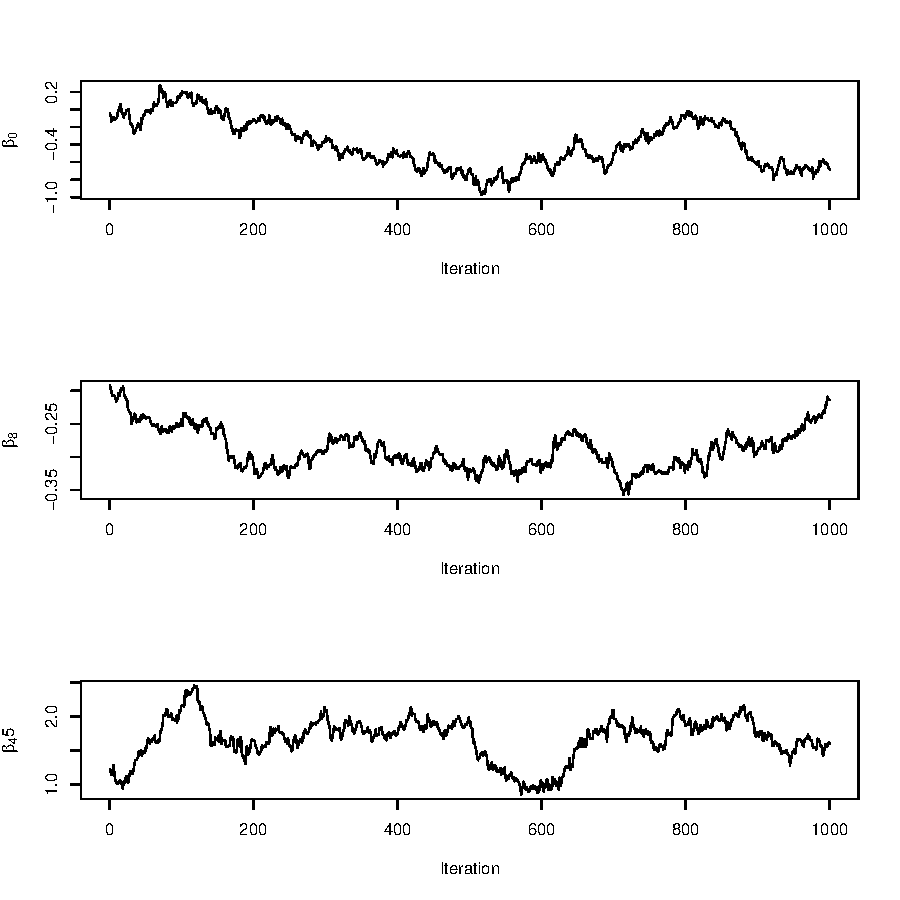
\includegraphics[width=1\textwidth]{traceplot_poisson_zip_da.pdf}
 \caption{Trace plots of three parameters from DA ZIP model}
 \end{subfigure}
  \hfill 
 \begin{subfigure}[b]{0.45\textwidth}
 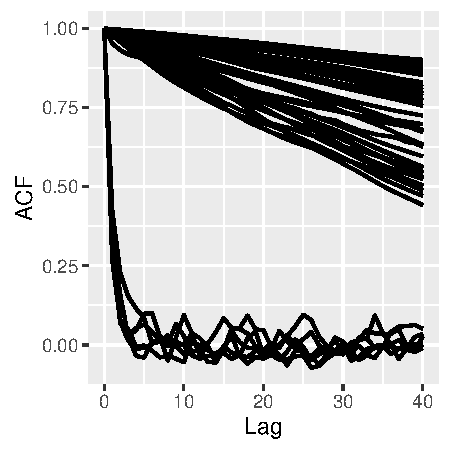
\includegraphics[width=1\textwidth]{poisson_zip_da_acf.pdf}
 \caption{Autocorrelation of all the 96 $\beta$'s from DA ZIP model.}
 \end{subfigure}  
 \caption{The hierarchy in the zero-inflated Poisson model does NOT help reduce the autocorrelation.}
 \end{figure}



\subsection{Goodness-of-Fit and Cross-Validation for Poisson Regression}


 \begin{figure}[H]
 % \centering
   \begin{subfigure}[b]{0.45\textwidth}
 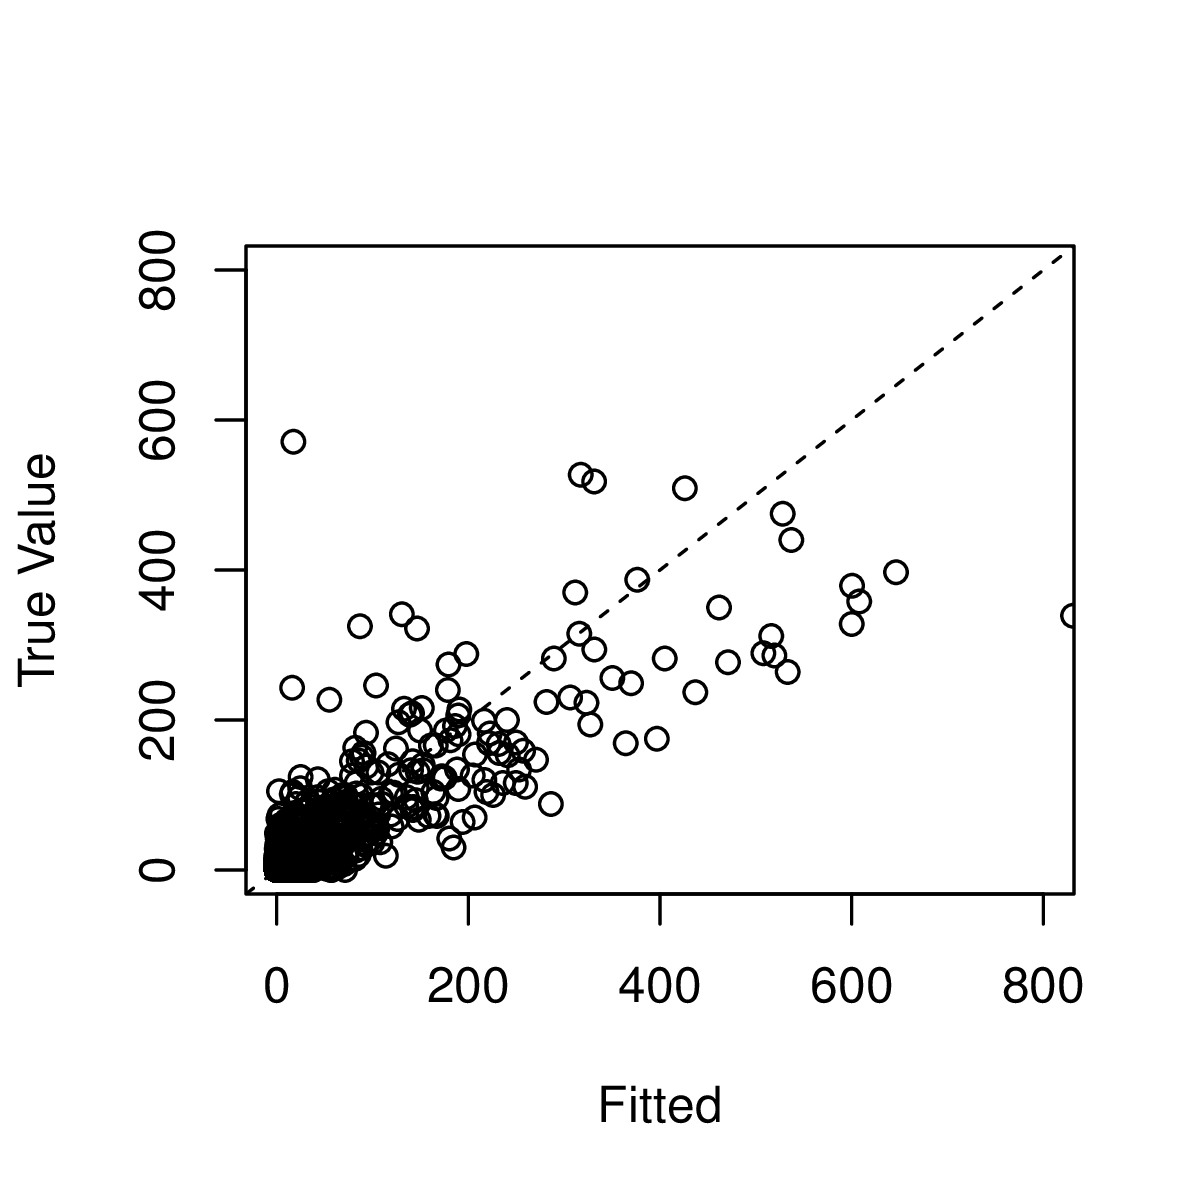
\includegraphics[width=1\textwidth]{poisson_fitting_da.png}
 \caption{Fitted vs true values using DA}
 \end{subfigure}
  \hfill 
 \begin{subfigure}[b]{0.45\textwidth}
 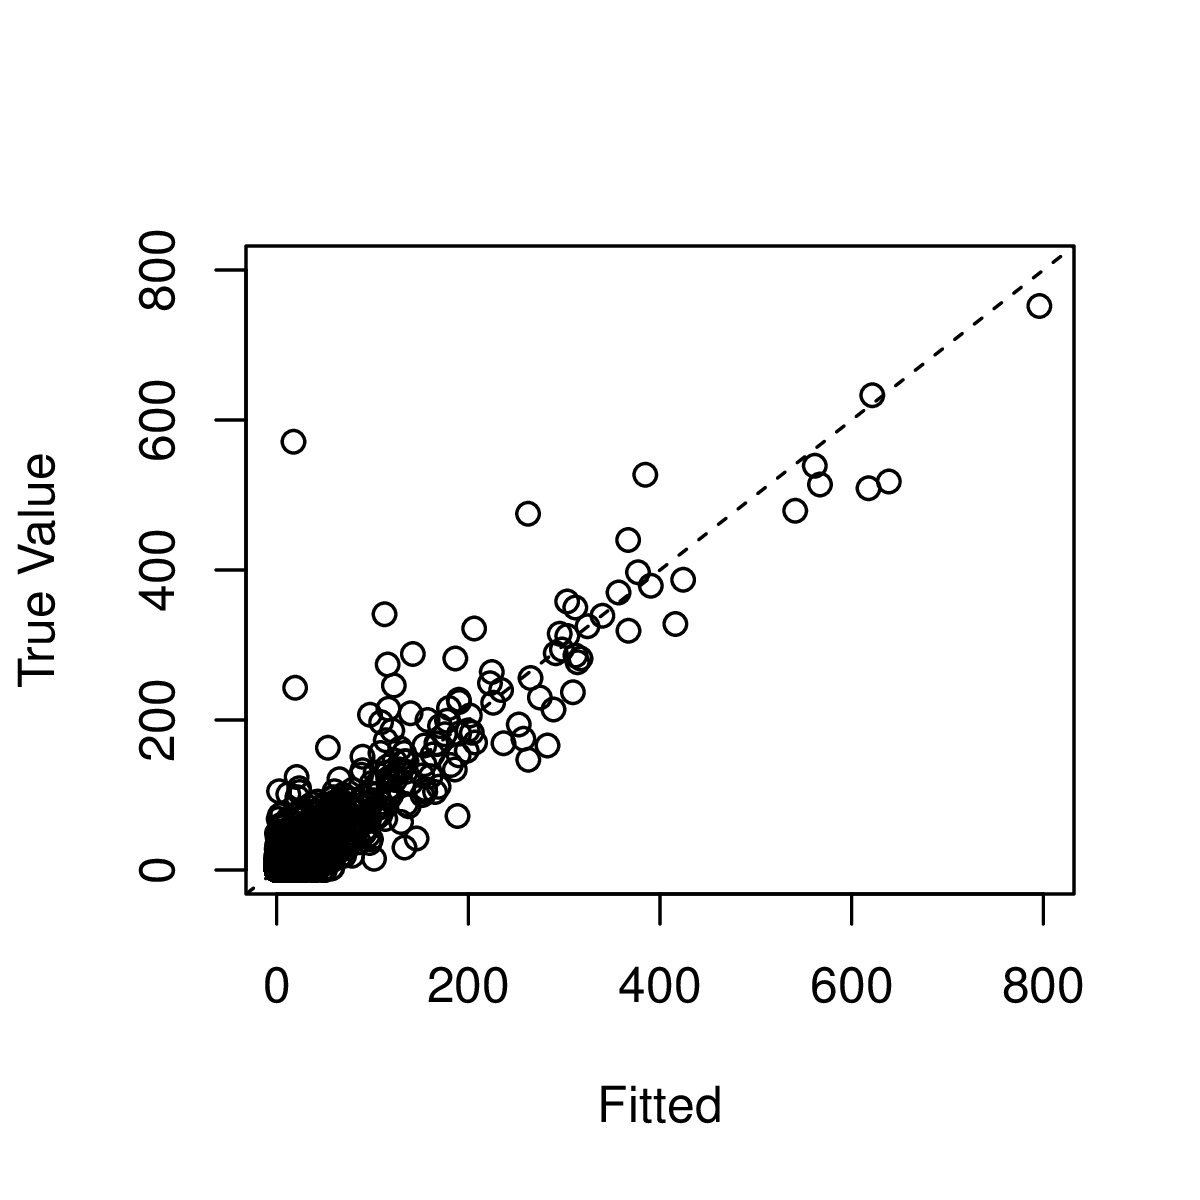
\includegraphics[width=1\textwidth]{poisson_fitting_ada.png}
 \caption{Fitted vs true values using CDA}
 \end{subfigure}  
   \begin{subfigure}[b]{0.45\textwidth}
 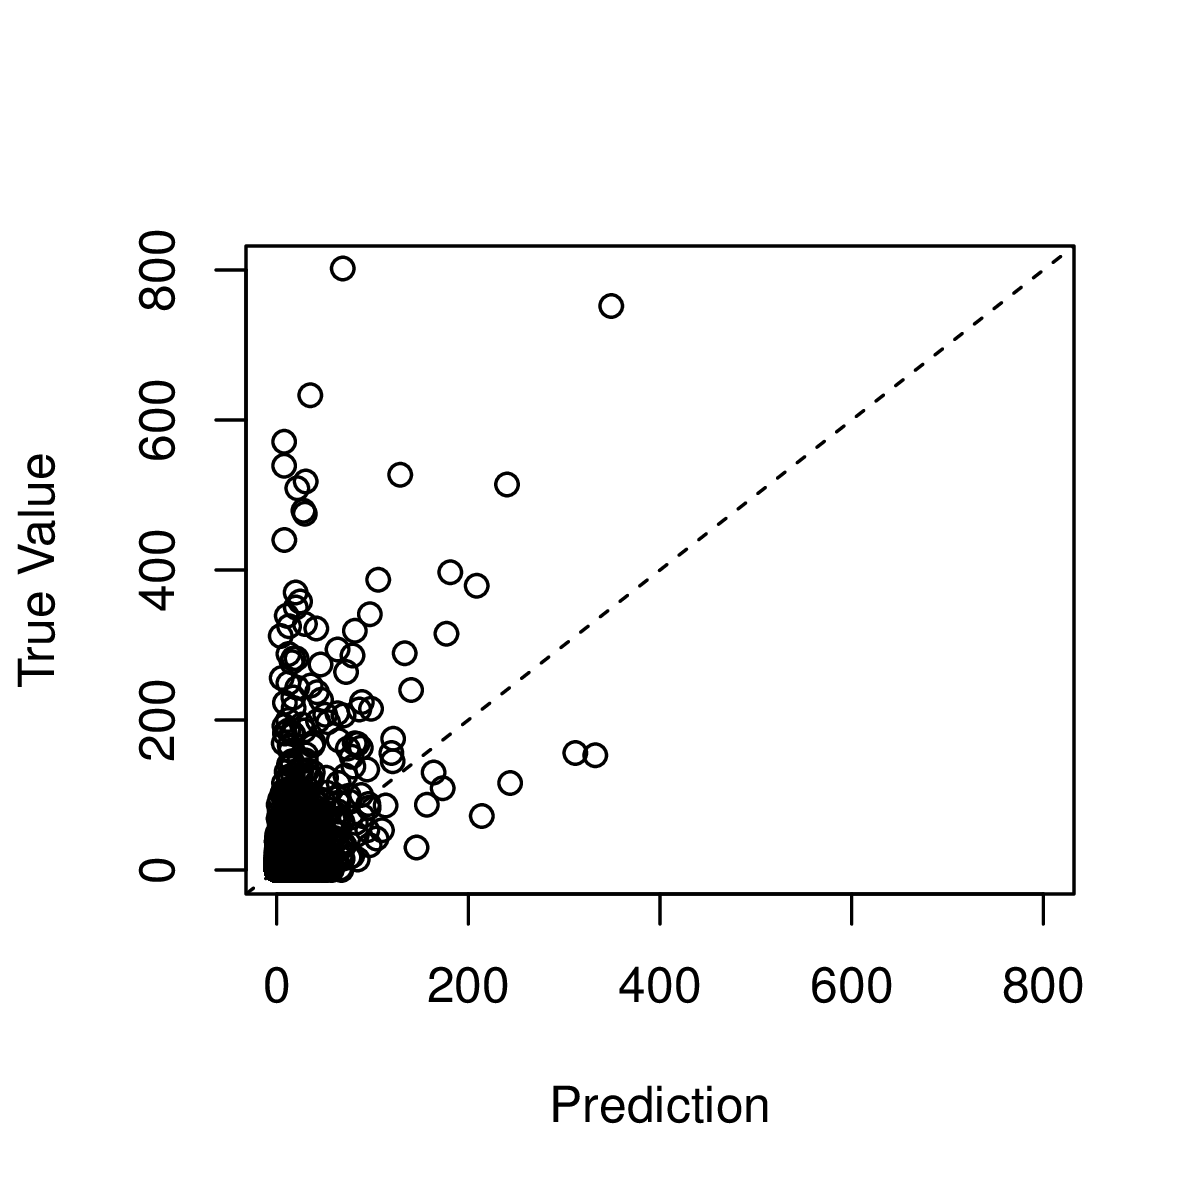
\includegraphics[width=1\textwidth]{poisson_cv_da.png}
 \caption{Prediction vs true values using DA}
 \end{subfigure}
  \hfill 
 \begin{subfigure}[b]{0.45\textwidth}
 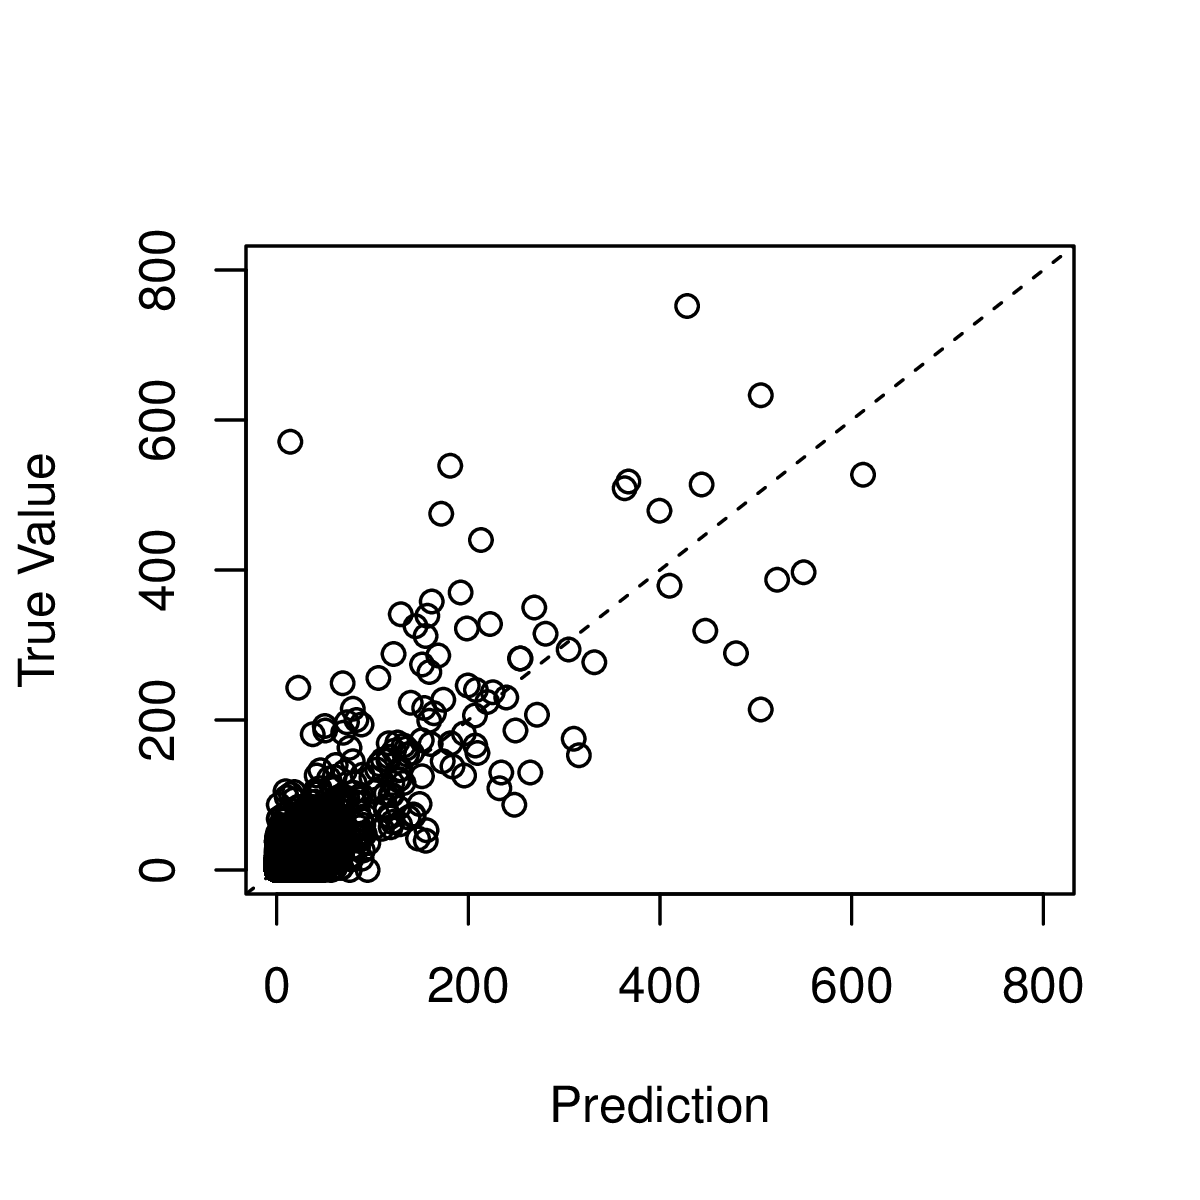
\includegraphics[width=1\textwidth]{poisson_cv_ada.png}
 \caption{Prediction vs true values using CDA}
 \end{subfigure} 
 \caption{The posterior estimates produced by CDA is better fitted to the data and have more accurate prediction than DA.}
 \end{figure}

 \subsection{Comparing posterior samples of CDA with HMC}


\begin{figure}[H]
 % \centering
   \begin{subfigure}[b]{0.45\textwidth}
 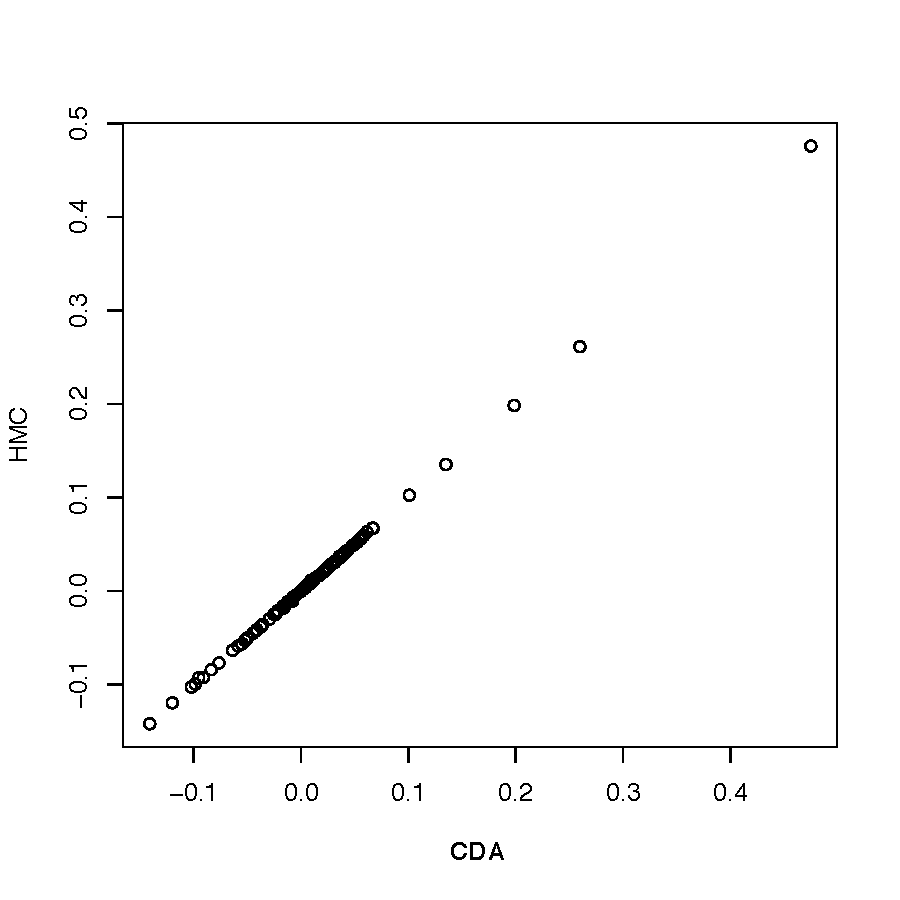
\includegraphics[width=1\textwidth]{CDAvsHMC_mean.pdf}
 \caption{Comparing posterior means for $\beta_1,\dots \beta_{95}$ from the HMC and CDA. The  RMSE between the two is $0.0007$.}
 \end{subfigure}
  \hfill 
 \begin{subfigure}[b]{0.45\textwidth}
 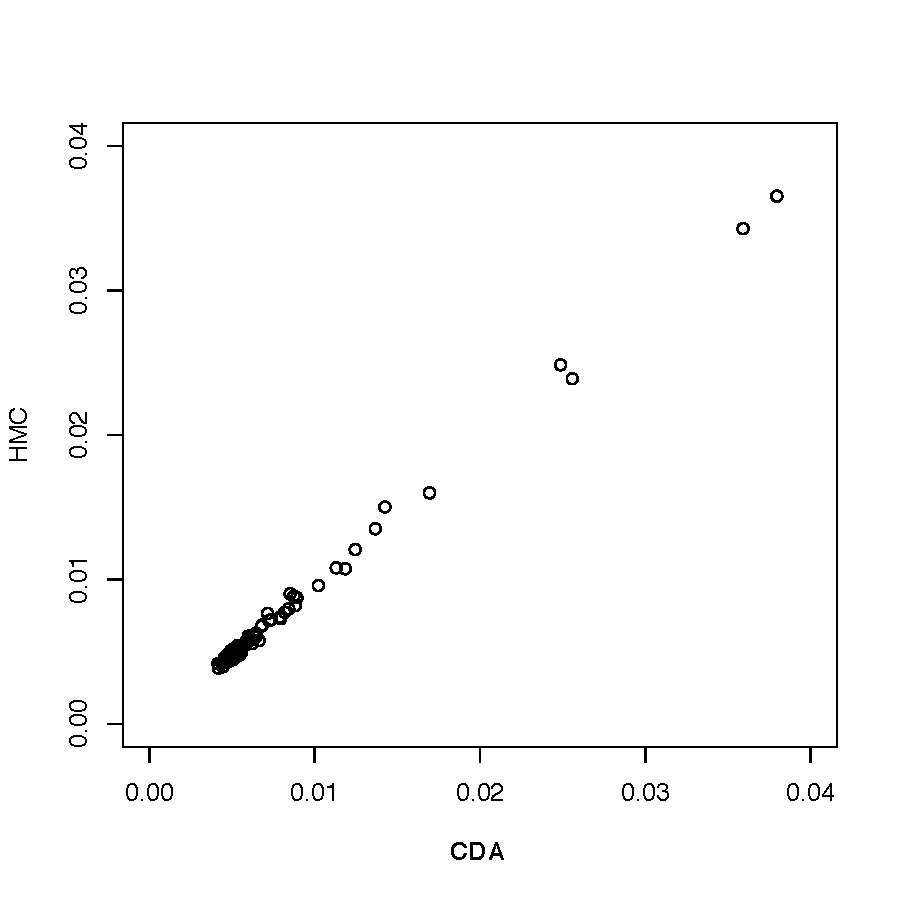
\includegraphics[width=1\textwidth]{CDAvsHMC_sd.pdf}
 \caption{Comparing posterior standard deviation for $\beta_1,\dots \beta_{95}$ from the HMC and CDA.  The  RMSE between the two is $0.0004$.}
 \end{subfigure}  
 \caption{The results from CDA and HMC agree very well.}
 \end{figure}

\subsection{Mixing of HMC}


 \begin{figure}[H]
 % \centering
   \begin{subfigure}[b]{0.45\textwidth}
 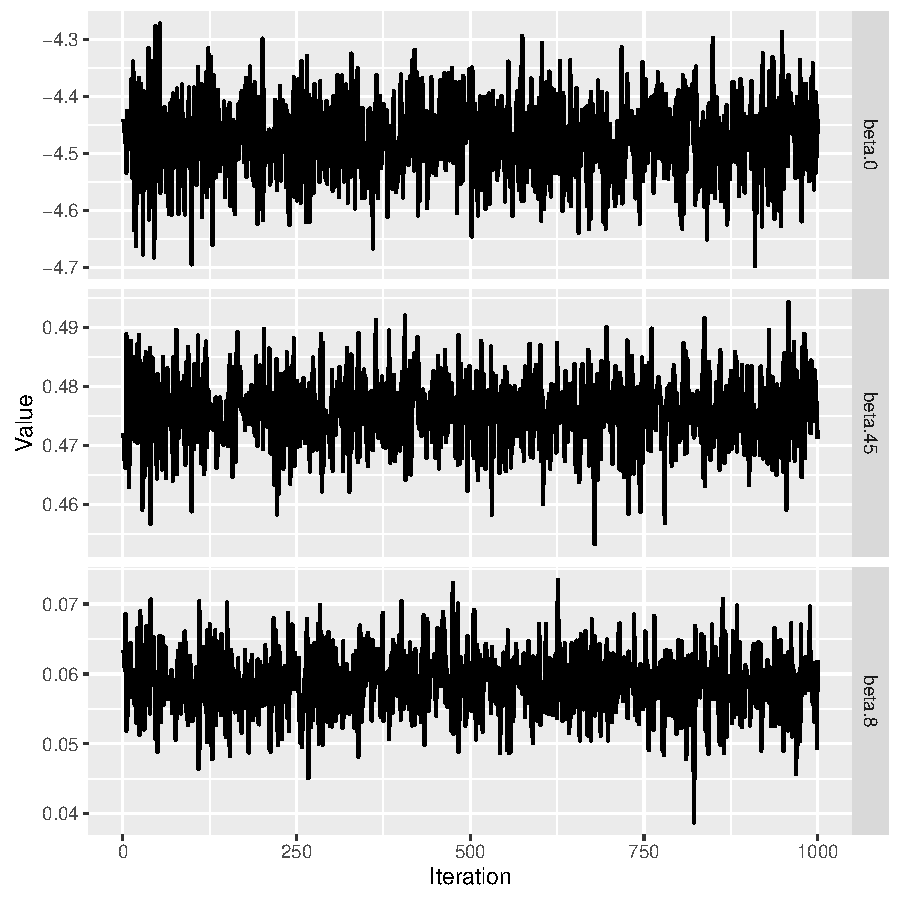
\includegraphics[width=1\textwidth]{traceplot_poisson_hmc.pdf}
 \caption{Traceplots}
 \end{subfigure}
  \hfill 
 \begin{subfigure}[b]{0.45\textwidth}
 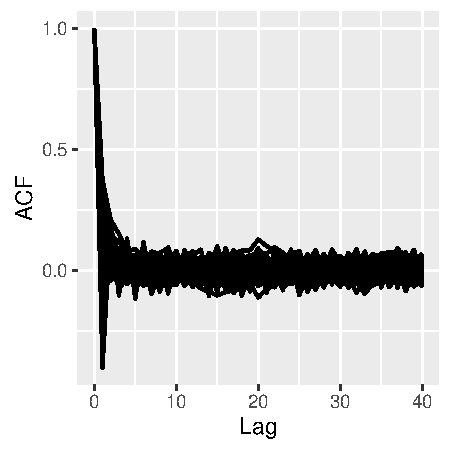
\includegraphics[width=1\textwidth]{poisson_hmc_acf.pdf}
 \caption{Autocorrelation}
 \end{subfigure}  
 \caption{The posterior estimates produced by HMC.}
 \end{figure}
 


 
\end{document}




